\documentclass[11pt,aps,preprint,nofootinbib,superscriptaddress,tightenlines]{revtex4-2}
\usepackage[T1]{fontenc}
\usepackage{amsmath,amssymb,mathtools}
\let\lambdabar\relax   % revtex defines it; newpxmath does too
\usepackage{newpxtext,newpxmath}
\usepackage{bm}
\usepackage[final]{microtype}
\usepackage{xcolor}
\usepackage{booktabs}
\usepackage{graphicx}
\usepackage{dsfont}
\usepackage[most]{tcolorbox}
\usepackage{algpseudocode}
\newcommand{\one}{\mathds{1}}
\newcommand{\avg}[1]{\langle #1\rangle}
\newcommand{\klab}{\mathcal B}
\definecolor{darkblue}{RGB}{20,60,140}
\definecolor{accent}{RGB}{30,80,150}
\definecolor{tint}{RGB}{243,246,251}
\newtcolorbox{algobox}[1]{enhanced, colback=tint, colframe=accent, boxrule=0.6pt, arc=2pt,
  left=6pt, right=6pt, top=4pt, bottom=4pt, fonttitle=\bfseries\small, coltitle=white,
  colbacktitle=accent, title={#1}, before skip=10pt, after skip=10pt}
\newtcolorbox{keyeq}{enhanced, colback=tint, frame hidden, borderline west={2pt}{0pt}{accent},
  sharp corners, left=4pt, right=4pt, top=0pt, bottom=0pt, before skip=6pt, after skip=6pt}
\usepackage[colorlinks=true,linkcolor=darkblue,citecolor=darkblue,urlcolor=darkblue]{hyperref}

\def\st{\begin{equation}}
\def\stp{\end{equation}}
\def\Eq#1{eq.~(\ref{#1})}
\def\Sect#1{Sect.~\ref{#1}}
\def\Fig#1{Fig.~\ref{#1}}
\def\Tab#1{Table~\ref{#1}}
\def\App#1{Appendix~\ref{#1}}
\def\tr{\operatorname{tr}}
\let\oldparagraph\paragraph
\renewcommand{\paragraph}{\par\bigskip\oldparagraph}


\begin{document}
\sloppy

\title{The S-scheme (state counting): development plan}
\author{D.~Teaney}
\affiliation{Department of Physics and Astronomy, Stony Brook University,
Stony Brook, New York 11794, USA}
\date{\today}

\begin{abstract}
This is the plan for implementing the state-counting renormalization of \nolinkurl{renorm3.tex}, which we call the S-scheme in the code.  The work has
two levels.  Level~1 is the single-particle scheme at one loop, for a constant speed of sound.  Level~2 adds the counterterm for the loop of the
particle positions.  Each level is implemented, tested, and then compared with the split scheme, first in equilibrium with hybrid Monte Carlo and then
in the dynamics.  The plan is written for the session at NERSC, which will do the work while the owner checks in from time to time.  It lists the
branches, the order of the work, the formulas to code, the tests, the campaigns, and the points where the owner must be asked.  Written 2026-11-25,
before any change to \nolinkurl{src/}.
\end{abstract}

\maketitle
\tableofcontents

%=============================================================================
\section{The goal}
\label{sec:goal}

The split scheme (\texttt{SPH\_RENORM=split}, \nolinkurl{step5_plan.tex}) removes the one-loop error of a single particle.  It keeps the part of the
counterterm that depends on the label in the measure, and it adds the rest to the Hamiltonian as an energy.  The S-scheme removes the same error in a
different way.  It defines the entropy of a particle as the logarithm of the number of states below its energy, and at one loop this puts the whole
counterterm into the entropy as an exact change of variables.  The theory is in \nolinkurl{renorm3.tex}, and the session should read that note first.

There are three reasons to prefer it.
\begin{enumerate}
\item Its single-particle error is smaller.  At rest the relative error of the pressure is $n\,c/S_{\rm t}^2$ with $c=1/12$ for $c_s^2=1/2$, which is
  $9\times10^{-7}$ at $S_{\rm t}=541$ and about $10^{-4}$ at $S_{\rm t}=54$ (\nolinkurl{renorm3.tex}, ``The accuracy of one loop'').
\item The weight of the votes needs no solve.  It follows directly from the target state of $(e,\bm m,V)$.
\item It extends to the loop of the positions.  The counterterm of level~2 is one more term in the entropy, of the same kind as the others.
\end{enumerate}
The aim is to show, with the same measurements as before, that level~1 does at least as well as split, and then that level~2 removes most of what
remains, which is the correction of the positions.  We expect the S-scheme to become the default, so the code is to be designed for it and not for
the older schemes.

\paragraph{The two levels.}
\begin{itemize}
\item \emph{Level 1} is state counting at one loop for one particle at fixed volume.  We assume a constant speed of sound (\texttt{ConstantCs2EOS}) in
  $d=2$, with neutral labels, $\mathcal B=0$.
\item \emph{Level 2} adds the positional counterterm $\omega$, built from the one-loop integral $I_0(\sigma)$ over the density modes and a term
  $a_2\nu_*^2$ whose coefficient is first zero and is then estimated from hybrid Monte Carlo.
\end{itemize}
The term of order $1/V$ in the single-particle expansion (\nolinkurl{renorm3.tex}, Appendix) is not part of this plan.

%=============================================================================
\section{For the NERSC session}
\label{sec:nersc}

The rules of \nolinkurl{CLAUDE.md} apply.  The points below are specific to this work.
\begin{enumerate}
\item \emph{Read first.}  Read \nolinkurl{docs/renorm3.tex} for the theory, \nolinkurl{docs/step5_plan.tex} for how the split scheme was implemented
  and measured, \nolinkurl{docs/split_dynamics.tex} for the dynamical runs, and \nolinkurl{nersc/LOG.md} for the state of the campaigns.
\item \emph{The reference implementation.}  \nolinkurl{examples/sscheme_ref.py} implements both levels in a few lines of Python, with the formulas of
  \Sect{sec:model1} and \Sect{sec:model2}.  It checks the closed forms against central differences of $H$ to $10^{-18}$.  Use it for reference values in
  the unit tests.  It is slow and is not a model for the Julia code.
\item \emph{Branches.}  Work only on the branches of \Sect{sec:branches}.  Do not commit to \texttt{split}, \texttt{legendre} or \texttt{main}.  Merge a
  feature branch into the integration branch \texttt{sscheme} only when its gate in \Sect{sec:branches} is passed.  Only the owner merges
  \texttt{sscheme} into \texttt{main}.
\item \emph{Checkout.}  Use a new worktree, \texttt{git worktree add \textasciitilde/stochastic-sph-sscheme sscheme}, and precompile there with
  \texttt{julia --project=nersc}.  Do not change the branch or the files of any existing worktree.
\item \emph{Design for the S-scheme.}  The S-scheme is expected to become the default, and the split and Legendre schemes to be removed later.  Write
  the code so that it is clear for the S-scheme (\Sect{sec:work1}~C).  The older schemes must keep running and pass their tests, but they need not
  stay bit-identical.  The default stays \texttt{split} until the owner changes it.
\item \emph{Budget.}  Tests and smoke runs go to \texttt{-q debug}.  Before each campaign, record the estimate in the log.  Ask the owner before
  submitting more than about 20 node-hours in one go.
\item \emph{Output.}  Each campaign has its own directory under \texttt{\$SCRATCH/sph/}.  In \nolinkurl{nersc/LOG.md} add one section per campaign of
  this plan and append only to it.
\item \emph{Check-ins.}  Stop and report to the owner at the points marked \textbf{Ask} below, and whenever a gate fails.  Otherwise continue to the
  next item.  At each check-in, update \Sect{sec:results} of this note with what was done and what was found.
\end{enumerate}

%=============================================================================
\section{Branches and merge points}
\label{sec:branches}

The integration branch \texttt{sscheme} is made from \texttt{split} at its present head, and this note is its first commit.  Each piece of work is a
feature branch made from \texttt{sscheme} and merged back with \texttt{--no-ff} when its gate is passed.
\begin{center}
\small
\begin{tabular}{llp{0.31\textwidth}p{0.27\textwidth}}
\toprule
branch & work & content & gate for the merge into \texttt{sscheme} \\
\midrule
\texttt{sscheme-maps} & \Sect{sec:work1} A, B, D & the quadrature decision, \nolinkurl{src/sscheme.jl}, \nolinkurl{test/testsscheme.jl} &
  unit tests of the maps pass \\
\texttt{sscheme-steps} & \Sect{sec:work1} C, E & the new particle field, the interface, both steps and hybrid Monte Carlo, timing, smoke runs &
  \texttt{test/run.sh all} passes, smoke runs agree with split within errors \\
\texttt{sscheme-eos} & \Sect{sec:work1} F & campaign \texttt{eos\_sscheme}, analysis, a new section of \nolinkurl{step5_plan.tex} &
  owner has read the comparison \\
\texttt{sscheme-dyn} & \Sect{sec:work1} G & campaign \texttt{hastings\_sscheme}, a new section of \nolinkurl{split_dynamics.tex} &
  owner has read the comparison \\
\midrule
\texttt{sscheme2-table} & \Sect{sec:work2} H & the kernel transform, the table of $I_0$ and its derivative, $\nu_*$, $\omega$ &
  reference values reproduced \\
\texttt{sscheme2-maps} & \Sect{sec:work2} I & $\omega$ in the maps, the setting for level~2, tests & as for \texttt{sscheme-steps} \\
\texttt{sscheme2-eos} & \Sect{sec:work2} J & campaign \texttt{eos\_sscheme2} with $a_2=0$ & owner has read the comparison \\
\texttt{sscheme2-dyn} & \Sect{sec:work2} K & campaign \texttt{hastings\_sscheme2} with $a_2=0$ & owner has read the comparison \\
\texttt{sscheme2-a2} & \Sect{sec:work2} L, M & the scan for $a_2$, the final equilibrium and dynamical runs & owner has read the comparison \\
\bottomrule
\end{tabular}
\end{center}
After \texttt{sscheme-dyn} is merged, level~1 is complete, and that is the first point at which the owner may merge \texttt{sscheme} into \texttt{main}.
Level~2 starts from the merged \texttt{sscheme}.  The second such point is after \texttt{sscheme2-a2}.  Campaign files, analysis scripts and figures are
committed on the branch of their campaign.  Raw data are never committed.

%=============================================================================
\section{Level 1: the model for a constant speed of sound}
\label{sec:model1}

This section gives the formulas to code.  They are those of \nolinkurl{renorm3.tex}, specialized to $p=A\,T_{\rm rel}^{\,n}$ in $d=2$, where
\st
n=1+q,\qquad q=\frac1{c_s^2},\qquad D=d+1=3 .
\stp

\paragraph{The two entropies of a particle.}  The particle carries two entropies, and the code keeps both.
\begin{itemize}
\item The \emph{label} $s$ is the variable of \nolinkurl{renorm3.tex}.  Its measure is the flat Liouville one, $e^{s}ds$, and the ideal step conserves
  it.  It is stored in \texttt{pa.s}.  It is not a physical entropy, and it can be negative.
\item The \emph{target entropy} $S_{\rm t}=\gamma\,s(T_{\rm rel})\,V$ is the entropy that the standard equation of state assigns to the particle's present
  $(e,\bm m,V)$.  It is stored in a new field, \texttt{pa.St}.  The ideal step changes it.  It is the entropy to use wherever the code needs a physical
  entropy of the particle, and it is the starting point of the next solve.
\end{itemize}
There is no third variable.  The stored variable of the split scheme, $s_{\rm eff}$ (the \texttt{u} of the code), is not used by the S-scheme.

\paragraph{The scheme.}  The label of a particle is its target entropy less the determinant term and the label term, all evaluated at the target
state of $(e,\bm m,V)$,
\begin{keyeq}
\st
s=S_{\rm t}-\Delta_\chi-\Delta_\ell,\qquad
\Delta_\chi=\frac D2\ln\big(2\pi V\gamma\,wT_{\rm rel}\big)+\tfrac12\ln a,\qquad
\Delta_\ell=1+\ln V+\ln\gamma-\ln T_{\rm rel} ,
\label{label}
\stp
\end{keyeq}
with $a\equiv q-v^2$ and $w=nA\,T_{\rm rel}^{\,n}$.  The logarithms contain dimensionful quantities in the units of the code.  A change of units adds a
constant to every label and has no other effect.

\paragraph{The state of the particle.}  Each term has its own slopes along the two modes,
\begin{align}
\Delta_p^{\chi}&=\frac D2\,(2+q-v^2)+\frac{v^2(1-v^2)}a, & \Delta_p^{\ell}&=-(1+v^2), \nonumber\\
\Delta_\theta^{\chi}&=\frac D2\,v-\frac{v\,(1-v^2)}a, & \Delta_\theta^{\ell}&=v ,
\label{slopes1}
\end{align}
and the shifts are built from their sums, $\Delta_p=\Delta_p^\chi+\Delta_p^\ell$ and $\Delta_\theta=\Delta_\theta^\chi+\Delta_\theta^\ell$,
\st
\epsilon_p=\frac{\Delta_p}{S_{\rm t}\,a},\qquad \epsilon_\parallel=\frac{\Delta_\theta}{S_{\rm t}},\qquad
\mathcal D\equiv1-(1+v^2)\,\epsilon_p+v\,\epsilon_\parallel .
\stp
With $T=T_{\rm rel}/\gamma$ the bare temperature of the target state, the temperature, the velocity and the pressure of the particle are
\begin{keyeq}
\st
T_a=\frac{\partial H}{\partial s}=\frac T{\mathcal D},\qquad
v_a=\frac{v\,(1-2\epsilon_p)+\epsilon_\parallel}{\mathcal D},\qquad
\frac{P_aV}{T_a}=\frac{S_{\rm t}}n-\Big(\frac D2+1\Big)+\frac1n\Big[\frac D2\,(2+q)-1\Big] .
\label{state1}
\stp
\end{keyeq}
The velocity $\bm v_a$ is along $\bm m$.  The energy is the target's, $H=V(w\gamma^2-p)$.  The quantity $\mathcal D$ is also the derivative of the
label with respect to the target entropy at fixed $\bm m$ and $V$, which is what the solve needs.

\paragraph{The weight of the votes.}  With the Liouville measure the weight of a particle in the energy is the label less $\ln T_a$,
\begin{keyeq}
\st
\texttt{vote\_entropy}(e,\bm m,V)=S_{\rm t}-\Delta_\chi-\Delta_\ell-\ln T_a .
\label{weight}
\stp
\end{keyeq}
All four terms follow from the target state of $(e,\bm m,V)$.  The weight needs no solve.

\paragraph{The domain.}  A state has a Hamiltonian when $\mathcal D>0$, so that $T_a>0$, and $|v_a|<1$.  Outside this domain the maps return a state
with no Hamiltonian, and the weight is $-\infty$.  There is no separate label boundary.

\paragraph{The relation to the split scheme.}  For a constant speed of sound the two terms combine into
\st
\Delta_\chi+\Delta_\ell=b\,\ln S_{\rm t}+\mathcal N\ln(\gamma V)+\tfrac12\ln\big(1-c_s^2v^2\big)+\text{const},\qquad
\mathcal N=1-d\,c_s^2,\qquad b=\frac D2+1-\mathcal N ,
\label{splitrel}
\stp
which are the label part and the dynamical part of the split scheme.  The split scheme keeps the first in the measure and adds the rest to the
energy.  The S-scheme puts all of it into the entropy.  This identity is used only as a test.

%=============================================================================
\section{Level 1: the work, in order}
\label{sec:work1}

\subsection{A. The single particle, before the code}

Extend \nolinkurl{examples/renorm_count_quadrature.py}, which is at rest, to a moving bath, following
\nolinkurl{examples/renorm_quadrature_split.py}.  Compute the relative errors of $E$, $M$, $P$, the violation $R$ of the density-frame relation and
$\mu/T$ for the S-scheme and for split, at $c_s^2=1/2$ and $1/4$, $s_a=16$, $54$, $541$, and $v=0$, $0.8$.  Use the domain of \Sect{sec:model1}.  The
expectation is that the S-scheme is as good as split or better at $s_a\ge54$.  Record the table in \Sect{sec:results}.
\textbf{Ask} the owner before going on if the S-scheme is worse than split anywhere at $s_a\ge54$, or if more than a few percent of the weight lies
outside the domain at $s_a=16$.

\subsection{B. The maps: \texorpdfstring{\nolinkurl{src/sscheme.jl}}{src/sscheme.jl}}

Write this file for the S-scheme alone.  It should not borrow the structure or the names of \nolinkurl{src/renorm_split.jl} or
\nolinkurl{src/renorm.jl}.  Its centre is one function that takes a target state and returns everything about the particle there, namely
$S_{\rm t}$, the label, the energy, $T_a$, $\bm v_a$, $P_a$, $\mathcal D$ and the weight, by \Eq{label}--\Eq{weight}.  Both maps call it.

\begin{algobox}{The map from the energy: $(e,\bm m,V)\to$ the state of the particle}
\begin{algorithmic}[1]
\State Find the target state $(T_{\rm rel},\bm v)$ with the standard equation of state.  For \texttt{ConstantCs2EOS} this is in closed form.
\State Evaluate the state of the particle there.  This gives the label $s$, $T_a$, $\bm v_a$ and the weight.
\State If $\mathcal D\le0$ or $|v_a|\ge1$, return a state with no Hamiltonian.
\end{algorithmic}
\end{algobox}

\begin{algobox}{The map from the label: $(s,\bm m,V)\to$ the state of the particle}
\begin{algorithmic}[1]
\State Start from the particle's present target entropy, \texttt{pa.St}.
\State Find the target state at $(S_{\rm t},\bm m,V)$ with the standard equation of state, and evaluate the state of the particle there.
\State Newton's step is $S_{\rm t}\leftarrow S_{\rm t}-\big(s(S_{\rm t})-s\big)/\mathcal D$.  Repeat from line 2 until the relative change is below $10^{-13}$.
\State Store the new $S_{\rm t}$ in \texttt{pa.St} and fill the fields: the energy, $T_a$, $\bm v_a$, $P_a$, and the target's rest-frame energy density
  and Lorentz factor.
\State If the iteration leaves the domain or does not converge, fall back to bisection on $S_{\rm t}$ between the edge of the domain and an upper
  bound, and count the event.  If no root exists, return a state with no Hamiltonian.
\end{algorithmic}
\end{algobox}

The reference implementation needs five or six Newton steps from a start that is off by thirty percent, and it will need fewer from the previous
value.  The maps must be robust first and fast second.  Keep counters of solves, iterations, fallbacks and states with no Hamiltonian.

\subsection{C. The design of the code}

The S-scheme is expected to become the default, and the split and Legendre schemes are expected to be removed later.  Design the code so that it is
clear and logical for the S-scheme.  Do not shape it around the older schemes.

\paragraph{The particle.}  Add the field \texttt{pa.St} for the target entropy (\Sect{sec:model1}).  With it the fields of a particle have one meaning
each.
\begin{itemize}
\item \texttt{pa.s} is the label, conserved by the ideal step and changed only by the viscous step.
\item \texttt{pa.St} is the target entropy of the present state.
\item \texttt{pa.T} is $T_a=\partial H/\partial s$, the velocity is $\bm v_a$ and the pressure is $P_a$.  These are the particle's own.
\item The target's $T_{\rm rel}$, Lorentz factor and rest-frame energy density are kept for the transport coefficients.
\end{itemize}
Go through the code and find every place that reads \texttt{pa.s} as a physical entropy, for example in a smoothed entropy density, in a division, or
in an output.  Each of these should read \texttt{pa.St}.  Find every use of the temperature and decide whether it wants $T_a$ or the target's.  Write the
list and the decisions in \Sect{sec:results}.

\paragraph{The interface.}  The two maps are the only place where the scheme enters, and the rest of the code should call them through one clear
interface.
\begin{itemize}
\item The ideal step and hybrid Monte Carlo call the map from the label.
\item The viscous step, the heat bath and the measurements call the map from the energy.  \texttt{vote\_entropy} is \Eq{weight} and calls no solve.
\item The starting guesses that the older schemes pass around (\texttt{VOTE\_GUESS}, the guess in \nolinkurl{src/hmc.jl}) are not needed.  The only
  starting point is \texttt{pa.St}.
\item A trajectory of hybrid Monte Carlo that leaves the domain is rejected, as now.
\end{itemize}
If the present interface (\texttt{particle\_forward}, \texttt{particle\_inverse}) is awkward for this, change it, and adapt the older schemes to the
new one.

\paragraph{The switch and the older schemes.}  \texttt{SPH\_RENORM=sscheme} selects the scheme at load time.  Its requirements are the energy
Hamiltonian, the number volume, $d=2$, the Liouville measure, and not the grid step.  The older schemes must keep running and pass their own tests,
because we may want to rerun a comparison.  They do not have to stay bit-identical.  If keeping one of them working makes the new code noticeably less
clear, \textbf{ask} the owner, who may decide to drop it.  The default is changed to \texttt{sscheme} by the owner after the comparisons of F and G.

\subsection{D. Tests: \texorpdfstring{\nolinkurl{test/testsscheme.jl}}{test/testsscheme.jl}}

\begin{enumerate}
\item The identities $\partial H/\partial s=T_a$, $\partial H/\partial\bm m=\bm v_a$ and $\partial H/\partial V=-P_a$ by central differences of $H$, to
  $10^{-9}$, at rest and in motion, for $c_s^2=1/2$ and $1/4$, and $S_{\rm t}=16$, $54$, $541$.
\item The map from the energy applied to the result of the map from the label returns the label to $10^{-13}$, and the reverse.
\item Reference values of the label, $T_a/T$, $v_a$ and $P_aV/T_a$ from \nolinkurl{examples/sscheme_ref.py} for the states it prints.
\item The identity \Eq{splitrel} to $10^{-12}$, with the constant taken from one state.
\item For the conformal fluid at rest the weight differs from that of \texttt{SPH\_RENORM=1} by a constant.
\item A state outside the domain returns no Hamiltonian from both maps, and the weight is $-\infty$.
\item Hybrid Monte Carlo has an energy error proportional to $\delta t^2$, and a reasonable acceptance.
\item \texttt{test/run.sh all}.  Every test passes with \texttt{SPH\_RENORM=sscheme}, the older schemes pass their own tests, and the regression with
  \texttt{SPH\_RENORM=0} is bit-identical to \texttt{main} unless a change was agreed with the owner.
\end{enumerate}

\subsection{E. Speed and smoke runs}

Time one update of \nolinkurl{examples/eos_measure.jl} at $h/a=2$ ($N=360$) and one step of the dynamics (\nolinkurl{examples/bench_step.jl}) for
split and for the S-scheme.  The stochastic step of the S-scheme should cost less than split's, since its weight needs no solve.  Then make smoke
runs at rest, $L=0.45$, $h/a=2$, $s_a=54$, two seeds, both values of $c_s^2$, against the numbers of split in \nolinkurl{step5_plan.tex}.  Finally make
one dynamical run with \nolinkurl{examples/stability.jl} to $t=20$ and check that $H$ does not drift.

\subsection{F. The equilibrium comparison: campaign \texttt{eos\_sscheme}}

Repeat the lines of \texttt{eos\_split} with \texttt{SPH\_RENORM=sscheme}.  These are $c_s^2\in\{1/2,1/4\}$, $s_a\in\{16,54,541\}$, $h/a\in\{2,3\}$,
$v\in\{0,0.8\}$, with 8 seeds of 300 updates, which makes 192 tasks.  The split campaign took 1.7 node-hours.  The split, tree-level and
\texttt{SPH\_RENORM=1} lines are reused from \texttt{eos\_split}.

The analysis is that of \nolinkurl{examples/eos_split.py} and \nolinkurl{examples/eos_compare.py} with one more Hamiltonian.  Add a new section,
``The S-scheme, level 1'', to \nolinkurl{step5_plan.tex}, with the same panels as its figures for split and the S-scheme side by side at $h/a=2$ and $3$.
Every caption begins with the campaign, the run sets and the commit.  On the panels for $E$ and $P$ at rest, add the prediction of the one-loop
correction of the positions as a dashed line,
\st
\frac{(P-p)\,\bar V}{T}=\frac{I_0+I_0'}{2\,\bar nh^2},\qquad \frac{(E-e)\,\bar V}{T}=\frac{q\,I_0'}{2\,\bar nh^2},\qquad I_0'\equiv\frac{dI_0}{d\ln\sigma} ,
\label{loopPE}
\stp
with $I_0$ of \Sect{sec:model2}.  These predictions already describe the offsets that split measured.  For Wendland C2 at $h/a=2$ and $c_s^2=1/4$ they
give $P/p-1$ of about $-5.1\%$ at $s_a=54$ and $-1.6\%$ at $s_a=541$, where split measured $-4.7\%$ and $-1.7\%$.  For $c_s^2=1/2$ at $s_a=541$ they give
$P/p-1=-1.2\%$ and $E/e-1=-0.4\%$, where split measured about $-1.3\%$ and $-0.4\%$.

What we want to learn is listed here.
\begin{itemize}
\item At $s_a\ge54$ the S-scheme and split should agree within errors, because both are dominated by the correction of the positions.
\item At $s_a=16$ the S-scheme should not be worse than split in $E$, $P$, $R$ and the susceptibilities.
\item There should be no failed solve, and the acceptance should not be below split's.
\end{itemize}
\textbf{Ask} the owner to read the new section before the branch is merged.

\subsection{G. The dynamical comparison: campaign \texttt{hastings\_sscheme}}

Repeat the split lines of \texttt{hastings\_bath} with \texttt{SPH\_RENORM=sscheme}.  These are the run sets \texttt{hs<sa>\_sp\_v<v>} and
\texttt{hq<sa>\_sp\_v<v>} with $s_a\in\{16,54\}$ and $v\in\{0,0.8\}$, 16 seeds of the full dynamics to $t=100$ and 16 chains of hybrid Monte Carlo,
which makes 128 runs.  All other settings are those of \texttt{hastings\_bath}.  That campaign took 3.9 node-hours for 256 runs.

Add a new section, ``The S-scheme, level 1'', to \nolinkurl{split_dynamics.tex}, with the following subset of its results, split and the S-scheme side by
side.
\begin{itemize}
\item The equal-time spectra of the dynamics against hybrid Monte Carlo of the same model.
\item The energy against time, to show that $H$ does not drift.
\item The advection speed and the damping rate of the shear mode from the fits.
\item The shear and sound correlators at $s_a=54$, at rest and at $v_0=0.8$.
\item The case that is open for split, $s_a=16$ at $v_0=0.8$.
\end{itemize}
The provenance rule of that note applies to every figure.  \textbf{Ask} the owner to read the new section before the branch is merged.

%=============================================================================
\section{Level 2: the model with the positional counterterm}
\label{sec:model2}

\paragraph{The loop of the positions.}  With the level~1 scheme the positions have the weight $\exp\sum_a[\lambda V_a-\ln(eV_a)]$ with
$\lambda=p\,\beta^0$.  In the Gaussian theory of \nolinkurl{partition.tex} their structure factor and its loop integral are
\st
\frac1{S(k)}=\big(1-\widetilde W\big)\big[1+(2\sigma-1)\widetilde W\big],\qquad
I_0(\sigma)=h^2\!\int\!\frac{d^2k}{(2\pi)^2}\,\ln S(k),\qquad \sigma=\lambda\,\bar V ,
\label{I0}
\stp
with $\widetilde W(k)$ the Fourier transform of the kernel, normalized to $\widetilde W(0)=1$.  The partition function per particle is then
$\sigma+I_0/(2\bar nh^2)$, and the second term is what the counterterm must cancel.

\paragraph{The counterterm.}  We subtract from the label term $\Delta_\ell$ a function of the particle's own target state and volume,
\begin{keyeq}
\st
\omega=a_1\,\nu_*+a_2\,\nu_*^2,\qquad
\nu_*\equiv-\frac{I_0(\bar\sigma)}{2\,a_1}\,\frac{V}{h^2},\qquad
\bar\sigma=\frac{p\,\gamma\,V}{T_{\rm rel}}=\frac{S_{\rm t}}n,\qquad a_1=\frac{\pi}{2\sin(2\pi/n_W)} .
\label{omega}
\stp
\end{keyeq}
Here $n_W$ is the power with which the kernel's transform falls, which is $5$, $7$ and $9$ for Wendland C2, C4 and C6 in $d=2$.  The first term of
$\omega$ is $-(V/2h^2)\,I_0(\bar\sigma)$ whatever $a_1$ is, so it is the one-loop counterterm exactly.  The variable $\nu_*$ is the number of stiff modes
per particle at large $\sigma$, and $a_2$ parametrizes what lies beyond one loop.  It is zero at first.  The label equation becomes
\begin{keyeq}
\st
s=S_{\rm t}-\Delta_\chi-\Delta_\ell+\omega(\bar\sigma,V) .
\label{label2}
\stp
\end{keyeq}

\paragraph{The slopes.}  With $\omega'\equiv a_1+2a_2\nu_*$, the two derivatives of the counterterm are
\st
\omega_\sigma\equiv\frac{\partial\omega}{\partial\ln\bar\sigma}\bigg|_V=\omega'\,\nu_*\,\frac{I_0'}{I_0},\qquad
\omega_V\equiv\frac{\partial\omega}{\partial\ln V}\bigg|_{\bar\sigma}=\omega'\,\nu_* .
\stp
Since $\partial\ln\bar\sigma/\partial\tau=q$, $\partial\ln\bar\sigma/\partial\theta=v$ and $\partial\ln\bar\sigma/\partial\ln V=1$, the formulas of
\Sect{sec:model1} hold with
\begin{keyeq}
\st
\Delta_p\to\Delta_p-a\,\omega_\sigma,\qquad \Delta_\theta\to\Delta_\theta-v\,\omega_\sigma,\qquad
\frac{P_aV}{T_a}\to\frac{P_aV}{T_a}+\omega_V+\frac{\omega_\sigma}n ,
\label{slopes2}
\stp
\end{keyeq}
and with $\omega$ added to the weight \Eq{weight}.  The reference implementation checks these against central differences of $H$.

%=============================================================================
\section{Level 2: the work, in order}
\label{sec:work2}

\subsection{H. The table of \texorpdfstring{$I_0$}{I0}}

\begin{enumerate}
\item Compute $\widetilde W(k)$ for the kernels of the code by a Hankel transform of the kernel as it is defined in \nolinkurl{src/sph.jl}, with its
  support and normalization.  The transform must be accurate where it is small.  A plain trapezoid sum loses accuracy beyond $kh\approx80$.  For
  Wendland C2, $\widetilde W\,(kh)^5\approx78$ from $kh\approx3$ on, with an oscillation of about ten percent.
\item Compute $I_0(\sigma)$ of \Eq{I0} on a grid in $\ln\sigma$ from $\sigma=1$ to $10^4$.  Integrate numerically to a large $kh$ and add the tail from
  the power law of $\widetilde W$ analytically.
\item Store $I_0$ and $I_0'=dI_0/d\ln\sigma$ in a table and interpolate with a spline whose derivative is consistent with the stored $I_0'$.
\item Reproduce the reference values for Wendland C2, which are $I_0=-0.979$, $-3.645$, $-3.874$, $-7.743$ and $-13.288$ at $\sigma=3.89$, $16.4$,
  $18$, $60$ and $179$.  As a check of the code, the same integral with $1/S=1+2\Pi\widetilde W-(2\Pi-\mathcal K)\widetilde W^2$, $\Pi=\sigma+3/2$ and
  $\mathcal K=3/2$ must give the values of \nolinkurl{partition.tex}, which are $-2.03$, $-4.14$ and $-13.43$ at $\sigma=3.89$, $16.4$ and $179$.
\item Provide $\nu_*$, $\omega$, $\omega_\sigma$ and $\omega_V$ of \Eq{omega} as functions of $(\bar\sigma,V)$, with $a_2$ a setting,
  \texttt{SPH\_SSCHEME\_A2}, whose default is zero.
\end{enumerate}

\subsection{I. The maps with \texorpdfstring{$\omega$}{omega}}

Level~2 is a setting of the same scheme, \texttt{SPH\_SSCHEME\_LEVEL=2}, and not a new one.  Both maps of \Sect{sec:work1}~B keep their structure.
The label is \Eq{label2}, the slopes are \Eq{slopes2}, and the derivative of the label with respect to $S_{\rm t}$ at fixed $\bm m$ and $V$ is still
$\mathcal D$, now with the new slopes.  Repeat the tests D1, D2, D3, D6, D7 and D8 with $\omega$ on, with $a_2=0$ and with $a_2=0.3$.  With the table replaced by
zero the maps must equal those of level~1 bit for bit.  Repeat the timing and the smoke runs of E.

\subsection{J. The equilibrium comparison with \texorpdfstring{$a_2=0$}{a2 = 0}: campaign \texttt{eos\_sscheme2}}

Repeat the campaign of F at level~2 with $a_2=0$.  Add a section ``The S-scheme, level 2'' to \nolinkurl{step5_plan.tex} with the
same panels, for split, level~1 and level~2.  The expectation is that the offsets of $E$ and $P$ that remain at $s_a\ge54$, which are the correction of
the positions, are reduced by a large factor, and by more at $h/a=3$ than at $h/a=2$.  Also measure two quantities that test the positions directly.
\begin{itemize}
\item The mean volume.  The condition $\ln\mathcal Z_N=p\,\beta^0L^2$ requires $\big\langle V_a\,(1+\partial\omega/\partial\bar\sigma)\big\rangle=\bar V$.
\item The structure factor at small $k$.  Its inverse extrapolated to $k=0$ is the stiffness of the labels, which should be small.
\end{itemize}
\textbf{Ask} the owner to read the section before the branch is merged.

\subsection{K. The dynamics with \texorpdfstring{$a_2=0$}{a2 = 0}: campaign \texttt{hastings\_sscheme2}}

Repeat the campaign of G with level~2 and $a_2=0$, and add the same subset of results to the section of \nolinkurl{split_dynamics.tex}, now with three
columns.  The counterterm changes the forces between particles, so check the drift of $H$ and the time step first, in a smoke run.

\subsection{L. The estimate of \texorpdfstring{$a_2$}{a2}}

The aim is to test that the remaining error depends on $\sigma$ and $h/a$ only through $\nu_*$, and to measure $a_2$.  If the model lacks a term
$a_2\nu_*^2$ in $\omega$, then with $a_2=0$ the remaining offsets at rest are
\begin{keyeq}
\st
\frac{(P-p)\,\bar V}{T}=-2a_2\,\nu_*^2\,\Big(1+\frac{I_0'}{I_0}\Big),\qquad
\frac{(E-e)\,\bar V}{T}=-2a_2\,\nu_*^2\,q\,\frac{I_0'}{I_0} .
\label{a2}
\stp
\end{keyeq}
Run hybrid Monte Carlo at rest with level~2 and $a_2=0$ on a grid of $s_a\in\{16,54,160,541\}$ and $h/a\in\{2,2.5,3,4\}$ at $c_s^2=1/2$, with enough
updates that the errors of $E$ and $P$ are a tenth of the offsets.  \textbf{Ask} the owner with the cost estimate before submitting.  Then do the
following.
\begin{enumerate}
\item Plot the two left sides of \Eq{a2}, each divided by its factor in $I_0'/I_0$, against $\nu_*^2$.  If the parametrization is right, all points
  fall on one line through the origin with slope $-2a_2$.
\item Fit $a_2$, with its error, from the points with $\nu_*<1/2$.  Report separately how the points at larger $\nu_*$ deviate.
\item Repeat a few points at $c_s^2=1/4$ to check that $a_2$ does not depend on the equation of state.
\item Rerun the grid with the fitted $a_2$ and confirm that the offsets are reduced.
\end{enumerate}
\textbf{Ask} the owner to read the result before going on.  If the points do not collapse, stop there and report.

\subsection{M. The final comparison}

With the fitted $a_2$, repeat the equilibrium campaign of J and the dynamical campaign of K, and add the fully renormalized results as a last column to
the sections of \nolinkurl{step5_plan.tex} and \nolinkurl{split_dynamics.tex}.

%=============================================================================
\section{Reporting}
\label{sec:reporting}

\begin{itemize}
\item \emph{This note.}  \Sect{sec:results} is the running record of the work.  For each item A to M it states what was implemented, what the tests
  gave, and any decision taken, with the commit.
\item \emph{The comparisons.}  The equilibrium results go into new sections of \nolinkurl{step5_plan.tex} and the dynamical ones into new sections of
  \nolinkurl{split_dynamics.tex}.  Existing sections of those notes are not edited.
\item \emph{Provenance.}  Every figure caption begins with the campaign, the run sets and the commit.  Tables go to \nolinkurl{docs/figs/} as
  \texttt{sscheme\_*.csv}.
\item \emph{The log.}  \nolinkurl{nersc/LOG.md} gets one section per campaign, with the job numbers and the node-hours.
\item \emph{Style.}  Full sentences, displayed equations, symbols defined, and no material that was not asked for.
\end{itemize}

%=============================================================================
\section{Open points for the owner}
\label{sec:open}

\begin{itemize}
\item The particle stores the label $s$ and the target entropy $S_{\rm t}$ (\Sect{sec:model1}).  The reported entropy per particle is the mean of
  $S_{\rm t}$.
\item The older schemes are kept running but are not kept bit-identical.  The owner decides when to remove them.
\item The constant $\mathcal B$ is zero throughout.  The stiffness that the loop induces is measured in J and is not corrected.
\item A variable speed of sound needs $\dot q$ in the slopes and is not part of this plan (\nolinkurl{renorm3.tex}).
\item A position update in the stochastic step is not part of this plan.
\item The form of the S-scheme (2026-11-26): the logarithm of the entropy in the measure, \Sect{sec:amend}.  The owner: the plain form, $F=1$, first.
\end{itemize}

%=============================================================================
\section{Level 1, amended: the logarithm of the entropy in the measure}
\label{sec:amend}

Added by the owner's desktop session on 2026-11-26, after the fold of item~E.  The owner has decided on this form as the default of the S-scheme.
The theory is in \nolinkurl{renorm3.tex}, Sect.~``The bounds, and the logarithm of the entropy in the measure''.  It is a fourth member of the family
of item~E2, and the one to implement first.  Items N1 to N5 below come before campaigns F and G.

\paragraph{Decision (owner, 2026-11-26).}  We first try the plain form, $F=1$.  The maps, the tests, the smoke runs and the campaigns are done for
the plain form only.  The form with the factor is kept in the single-particle quadrature of N1 as a comparison, and in the reference script.  It is
implemented in \nolinkurl{src/} only if N1 or the campaigns show that the plain form loses accuracy in motion, and only after asking the owner.

\paragraph{The idea.}  The fold comes from the term $(D/2+1)\ln S_{\rm t}$ of $\Delta$.  The ideal step preserves $d\bm x\,d\bm m$ and conserves the
label, so any positive function of the label may stand in the measure.  We therefore move that term into the measure, as split does with $b\ln u$, and
keep the rest of $\Delta$ in the label, where it is inverted exactly as in the S-scheme.  What remains in the Hamiltonian is a function of
$T_{\rm rel}$ and the bounded sound factor.  It has no explicit volume, it is almost independent of the velocity, and its slope has the safe sign.

\paragraph{The model for a constant speed of sound.}  With $\beta=D/2+1$ and $T_0$ the rest-frame temperature of the nominal state of the run
(\texttt{trel\_of\_srel} of \texttt{SR\_SREL0}),
\begin{keyeq}
\st
\begin{gathered}
s=S_{\rm t}-F\,\Delta^H,\qquad \Delta^H=-(q-d)\ln\frac{T_{\rm rel}}{T_0}+\tfrac12\ln\big(1-c_s^2v^2\big),\\
\rho(s)=e^{\,s}s^{-\beta}\Big(1-\frac\beta s\Big)\quad(s>\beta) .
\end{gathered}
\label{amend}
\stp
\end{keyeq}
There are two forms.  In the plain form $F=1$.  In the form with the factor, $F=(S_{\rm t}+2\beta)/(S_{\rm t}+\beta)$, which restores the agreement
with \Eq{label} to order $1/S_{\rm t}^2$.  With
\st
\begin{gathered}
\Delta_p^H=-(q-d)+\frac{v^2(1-v^2)}{a},\quad \Delta_\theta^H=-\frac{v(1-v^2)}{a},\\
\epsilon_p=\frac{F\Delta_p^H}{S_{\rm t}a},\quad \epsilon_\parallel=\frac{F\Delta_\theta^H}{S_{\rm t}},\quad
\kappa=1+\frac{\beta\,\Delta^H}{(S_{\rm t}+\beta)^2}
\end{gathered}
\stp
(and $\kappa=1$ in the plain form), the state of the particle is
\st
\begin{gathered}
T_a=\frac{T}{\mathcal D},\qquad \mathcal D=\kappa-(1+v^2)\epsilon_p+v\,\epsilon_\parallel,\\
v_a=\frac{v(\kappa-2\epsilon_p)+\epsilon_\parallel}{\mathcal D},\qquad
\frac{P_aV}{T_a}=\frac{\kappa\,S_{\rm t}-F\,(q-d)}{q+1} .
\end{gathered}
\label{amendstate}
\stp
The weight of the votes, of the heat bath and of the equilibrium draw is
\st
\ln\rho(s)-\ln T_a=s-\beta\ln s+\ln\Big(1-\frac\beta s\Big)-\ln T_a ,
\label{amendweight}
\stp
and it is $-\infty$ for $s\le\beta$.  The reference implementation is \texttt{state\_m} in \nolinkurl{examples/sscheme_ref.py}.

\paragraph{N1. The single particle.}  Add the two forms to \nolinkurl{examples/renorm_quadrature_sscheme.py} (models \texttt{sscheme-m} and
\texttt{sscheme-mf}), with the measure $\rho(s)$ in place of $e^s$ and the labels restricted to $s>\beta$.  Repeat Table~\ref{tab:A} for both, with
$s_a=30$ added.  Report $E$, $p$, $R$, and the weight of the tree-level particle below the bound.  The expectation is that the form with the factor
reproduces the S-scheme columns at $s_a\ge54$, and that the plain form differs from them in motion by an amount of the size of split's errors.

\paragraph{N2. The maps.}  One setting selects the form, \texttt{SPH\_SSCHEME\_FORM} with the values \texttt{full} (\Eq{label}, the present code)
and \texttt{measure} (the plain form, to become the default).  The value \texttt{measure-f} (with the factor) is reserved and not implemented now.  \texttt{sscheme\_state} returns the same fields, computed from \Eq{amend} and
\Eq{amendstate}, and the weight \Eq{amendweight}.  The map from the label is the same Newton iteration on $S_{\rm t}$ with the derivative
$\mathcal D$.  The level~2 counterterm will enter as $\Delta^H\to\Delta^H-\omega$, so keep $\Delta^H$ and its slopes in one place.  The weight is the
only place where $\rho$ enters.  The ideal step never evaluates it.

\paragraph{N3. Tests.}  Repeat tests 1 to 3 of item~D against \texttt{state\_m} for the plain form.  Add three tests.  (i) On a grid of $(\bm m,V)$ the
label increases with $S_{\rm t}$ for every $S_{\rm t}$ whose label is above $\beta$, and every label above $\beta$ has a root.  (ii) For a small system
the Jacobian determinant of one ideal step in $(\bm x,\bm m)$ at fixed labels is one, by finite differences.  This tests that $\bm v_a$ and $P_a$ are
the derivatives of one Hamiltonian, whatever the form.  (iii) Test~7 at $s_a=16$, both $c_s^2$: the expectation is the acceptance of split, with no
trajectory leaving the domain.

\paragraph{N4. Smoke runs and the decision.}  Repeat the smoke runs of item~E at $s_a=16$ and $54$, at rest and at $v_0=0.8$, for the plain form.  Record
the fraction of particles with $P_a<0$ and the number of proposals rejected at the bound.  \textbf{Ask}: show the owner N1 and N4 before the campaigns.

\paragraph{N5. The campaigns.}  Campaigns F and G then run with the plain form, and include $s_a=16$.  The sensitivity study of item~E2 becomes a
variation of this form: $\beta=D/2$, $b$ and $D/2+1$, with and without the factor, and a bound of the measure placed above $\beta$.

\paragraph{The bounds to expect} (\nolinkurl{renorm3.tex}, the table of bounds).  Above $s=\beta$ the temperature is positive and $|v_a|<1$ at every
velocity for $c_s^2=1/2$, $1/3$, $1/4$ and $1/6$ in the scans of the desktop session.  The pressure is positive for $S_{\rm t}>q-d$, which is below the
bound of the measure for $c_s^2\ge1/4$ in the plain form.  With the factor at $c_s^2=1/4$ and $s_a=16$ the pressure was negative up to the label
$2.8$, slightly above the bound.

\paragraph{Level 2.}  The model of \Sect{sec:model2} is unchanged except that $\omega$ is subtracted from $\Delta^H$ instead of $\Delta_\ell$.  The
slopes \Eq{slopes2} apply to $\Delta_p^H$ and $\Delta_\theta^H$.  Since $\omega$ grows with $S_{\rm t}$, the test (i) of N3 must be repeated with
$\omega$ before the level~2 runs.

%=============================================================================
\section{Results}
\label{sec:results}

To be filled by the session, item by item.

\subsection*{A. The single particle (2026-11-25, branch \texttt{sscheme-maps}, commit 8aaccb6)}

\nolinkurl{examples/renorm_quadrature_sscheme.py} adds the S-scheme to the models of \nolinkurl{examples/renorm_quadrature_split.py} and
integrates $Z_1(T,\bm v,V)$ with the label gas for the tree level, split (the model \texttt{step5-du0}, which is \texttt{SPH\_RENORM=split}) and the
S-scheme.  The quadrature now runs in $\ln T$ and the rapidity vector.  In the variables $(T,\bm v)$ of the split script the weight of both
renormalized models rises toward the light cone, because the volume element does, so there is no peak near the bath state to centre the Gaussian
grid on.  That grid failed at $c_s^2=1/2$, $s_a=16$, $v=0.8$, and at $s_a=54$, $v=0.8$ it missed a tail worth a few $10^{-4}$ in $E$.  In the new
variables the results converge to about $10^{-6}$ with $201^3$ points over $\pm26\sigma$.  Table~\ref{tab:A} gives the relative errors of $E$ and $p$ and
the violation $R$ of the Density Frame relation $M=v(E+pV)$ (the error of $M$ follows $E$).  The rows are in \nolinkurl{docs/figs/sscheme_quadrature.csv}.

\begin{table}[h]
\caption{Item A: the single particle by quadrature (\nolinkurl{examples/renorm_quadrature_sscheme.py}, commit 8aaccb6), split against the
S-scheme.  Relative errors of the energy and the pressure, and $R=M/[v(E+pV)]-1$.}
\label{tab:A}
\small
\begin{tabular}{cccrrrrrr}
\toprule
 & & & \multicolumn{3}{c}{split} & \multicolumn{3}{c}{S-scheme} \\
$c_s^2$ & $s_a$ & $v$ & $E$ & $p$ & $R$ & $E$ & $p$ & $R$ \\
\midrule
$1/2$ & 16 & 0 & $3.9\times10^{-2}$ & $3.9\times10^{-2}$ & & $4.2\times10^{-2}$ & $4.2\times10^{-2}$ & \\
 & 16 & 0.8 & $3.9\times10^{-2}$ & $4.0\times10^{-2}$ & $-3.1\times10^{-4}$ & $4.0\times10^{-2}$ & $3.9\times10^{-2}$ & $4.2\times10^{-4}$ \\
 & 54 & 0 & $2.4\times10^{-4}$ & $2.4\times10^{-4}$ & & $1.8\times10^{-4}$ & $1.8\times10^{-4}$ & \\
 & 54 & 0.8 & $6.9\times10^{-4}$ & $8.0\times10^{-4}$ & $-5.2\times10^{-5}$ & $2.8\times10^{-4}$ & $2.4\times10^{-4}$ & $1.9\times10^{-5}$ \\
 & 541 & 0 & $9.7\times10^{-7}$ & $9.7\times10^{-7}$ & & $9.2\times10^{-7}$ & $9.2\times10^{-7}$ & \\
 & 541 & 0.8 & $6.1\times10^{-6}$ & $7.2\times10^{-6}$ & $-5.8\times10^{-7}$ & $2.3\times10^{-6}$ & $2.0\times10^{-6}$ & $1.3\times10^{-7}$ \\
$1/4$ & 16 & 0 & $8.5\times10^{-2}$ & $1.0\times10^{-1}$ & & $8.0\times10^{-2}$ & $7.3\times10^{-2}$ & \\
 & 16 & 0.8 & $8.0\times10^{-2}$ & $9.6\times10^{-2}$ & $4.1\times10^{-4}$ & $7.3\times10^{-2}$ & $6.3\times10^{-2}$ & $1.5\times10^{-3}$ \\
 & 54 & 0 & $5.3\times10^{-4}$ & $2.4\times10^{-3}$ & & $5.8\times10^{-4}$ & $5.7\times10^{-4}$ & \\
 & 54 & 0.8 & $-4.4\times10^{-4}$ & $1.0\times10^{-3}$ & $3.5\times10^{-5}$ & $4.4\times10^{-5}$ & $-1.0\times10^{-4}$ & $7.6\times10^{-5}$ \\
 & 541 & 0 & $3.3\times10^{-6}$ & $2.1\times10^{-5}$ & & $3.3\times10^{-6}$ & $3.3\times10^{-6}$ & \\
 & 541 & 0.8 & $-3.7\times10^{-6}$ & $9.5\times10^{-6}$ & $3.2\times10^{-7}$ & $-1.3\times10^{-7}$ & $-1.5\times10^{-6}$ & $6.9\times10^{-7}$ \\
\bottomrule
\end{tabular}
\end{table}

At $s_a\ge54$ the S-scheme is as good as split or better in $E$ and $p$, by up to a factor of ten at $c_s^2=1/4$, $s_a=54$, $v=0.8$.  Its $R$ is of
the same size as split's, larger by a factor of two to four in some rows; all are below $10^{-4}$.  At rest the S-scheme has $E$ and $p$ equal, as
\nolinkurl{renorm3.tex} predicts for one loop, and at $s_a=541$ they agree with $n\,c/S_{\rm t}^2$.  At $s_a=16$ both schemes are off by 4 to 10
percent, about the same.  The weight of the tree-level particle that lies outside the S-scheme's domain at $s_a=16$ is $1$--$9\times10^{-4}$, below
the few percent at which the plan asks; 3.5 to 5 percent of the S-scheme's own weight lies within 3 of the boundary in $S_{\rm t}$.  The owner was
shown the table and agreed to go on.

\subsection*{B. The maps (commit 8aaccb6)}

\nolinkurl{src/sscheme.jl}.  The centre is \texttt{sscheme\_state}$(T_{\rm rel},\gamma v,V)$, which returns the label, $S_{\rm t}$, $H$, $T_a$,
$v_a$, $P_a$, $\mathcal D$ and the weight by \Eq{label}--\Eq{weight}.  For \texttt{ConstantCs2EOS} both target inversions are one-dimensional: from
the energy the rest-frame energy density is in closed form, and from $(S_{\rm t},|\bm m|,V)$ the temperature solves
$(nAV)^2T_{\rm rel}^{2n-4}(T_{\rm rel}^2+|\bm m|^2/S_{\rm t}^2)=S_{\rm t}^2$, monotonic, by Newton in $\ln T_{\rm rel}$.  The map from the label iterates
on $S_{\rm t}$ from the previous value, 2.4 steps per solve in the tests, with a bisection on $S_{\rm t}$ as the fallback.  The file is loaded but not
yet called by the steps.

\subsection*{D. Tests 1--6 (commit 8aaccb6)}

\nolinkurl{test/testsscheme.jl}, on the login node in 9~s, all passing.  The derivatives of $H$ by fourth-order central differences agree with $T_a$,
$v_a$ and $P_a$ to $3\times10^{-10}$ or better.  The two maps invert each other to $2\times10^{-15}$.  The reference values of
\nolinkurl{examples/sscheme_ref.py} are reproduced to $10^{-15}$.  The relation to split, \Eq{splitrel}, holds to $6\times10^{-14}$, and at rest the
weight differs from that of \texttt{SPH\_RENORM=1} by a constant to $3\times10^{-13}$.  Test 7 (hybrid Monte Carlo) comes with item C.

\subsection*{C. The design (branch \texttt{sscheme-steps}, commit 3fa7a3e; in progress)}

\paragraph{The volume is stored.}  The code kept the number volume as \texttt{S\_smooth}$\,=s_an_a$ and recovered $V_a=s_a/S_a$, $\bm m_a/V_a$, the
energy $s_a\,(H/s)_a$ and the velocity $(v/S)_aS_a$ through the label.  The label of the S-scheme can be zero or negative, so (owner, 2026-11-25) the
particle now stores four more fields, filled by every scheme: \texttt{pa.V} (set by the density pass), \texttt{pa.H}, \texttt{pa.v} and \texttt{pa.St}.  At the
tree level, split and Legendre they are filled with the expressions the code used before, so the regression against \texttt{main} should stay
bit-identical; the code reads the fields in place of those expressions.  With the S-scheme the density pass sets $V_a=1/n_a$ and
$\bm M_a=\bm m_an_a$ directly, and \texttt{S\_smooth} is the target's entropy density $S_{\rm t}/V$.

\paragraph{The uses of the label as an entropy.}  The helper \texttt{entropy\_of(pa)} returns $S_{\rm t}$ with the S-scheme and the label otherwise.
It is used by the cut of the diffusive time step (\texttt{compute\_dt}), the entropy Fourier mode of the records (\nolinkurl{measure.jl}) and the
spread of the entropies (\nolinkurl{examples/equilibrium.jl}).  The set-up (\texttt{setup\_ic}) gives each particle the target entropy $S(\bm x)V$; with
the S-scheme \texttt{sscheme\_labels!} replaces it by the label of the state with that target entropy, momentum and volume.  The set-ups of
\nolinkurl{examples/equilibrium.jl} that rescale the label as an entropy (\texttt{SR\_JITTER}, \texttt{SR\_POSITIONS=poisson}) stop with a message;
the default start (lattice, then hybrid Monte Carlo and the equilibrium draw) sets the labels through the inverse map.  Not changed: the
gradient-corrected conversion map and the smoothed Hamiltonian, which the S-scheme does not support (\texttt{check\_sscheme}).

\paragraph{The temperatures and velocities.}
\begin{itemize}
\item The ideal step and hybrid Monte Carlo use the particle's own $T_a$ (\texttt{pa.T}), $\bm v_a$ (\texttt{pa.v}, also \texttt{pa.dotx}) and $P_a$
  (\texttt{pa.p}, in the force $P_aV_a^2$).
\item The votes use the weight $s-\ln T_a$ from the map from the energy, and the stochastic step's $\bm v_a/T_a$ is the particle's.
\item The transport coefficients and the comoving structures of the viscous step use the target state: $T_{\rm rel}$ (\texttt{target\_trel}), the
  rest-frame energy density (\texttt{pa.e}) and the target's velocity, in \texttt{build\_stars} and, for the Hastings correction, in
  \texttt{star\_coef} at each proposal, so that both evaluate the coefficients at the same state.  The time step uses the target's $T_{\rm rel}$.
\end{itemize}
The energy measured by the drivers is $\sum_aH_a$ and the virial uses $P_aV_a^2$ and $\bm v_a\bm m_a$.

\paragraph{Test 7.}  \nolinkurl{test/testsscheme_hmc.jl}: at $s_a=54$, $h/a=2$, both $c_s^2$, the energy error of a trajectory falls by 16.1 when
$\delta t$ is halved twice, 5 of 5 updates are accepted, about $9\times10^4$ solves from the label take 1.7 Newton steps each with no fallback and no
state outside the domain.

\paragraph{The test suite} (interactive 62000863, \texttt{test/run.sh all} against \texttt{main} 00064e7 at the default scheme, and \texttt{unit},
\texttt{load} with \texttt{SPH\_RENORM=sscheme}; commit 578487e, whose \nolinkurl{src/} and \nolinkurl{test/} are those of 3fa7a3e).  All unit tests,
including \texttt{testsscheme} and \texttt{testsscheme\_hmc}, the physics tests, the load test and three of the five regression items pass; every
script loads with the S-scheme.  The equilibrium driver (at rest and boosted) has a bit-identical trajectory, and three diagnostics differ because they
now read the stored fields: the energy series $H(t)$ (before, $s_a\,(H/s)_a$ mixed the labels after the stochastic step with $(H/s)_a$ from before it, a
noise of $10^{-5}$ in $\Delta H/H$; now $10^{-7}$), and KE/eq and the volume spread (before, $s_a/S_a$ with a stale $S_a$; $10^{-6}$ at rest, 0.3 percent
boosted).  The known differences \texttt{hast\_lq\_*} remain.  The tree-level unit tests fail when \texttt{SPH\_RENORM=sscheme} is forced on them, as
they did for split; they set \texttt{SPH\_RENORM=0} themselves in the default run.

\subsection*{E. First smoke runs (2026-11-25, debug 61997657, 61997960; commit 3fa7a3e)}

\paragraph{Dynamics.}  \nolinkurl{examples/equilibrium.jl}, $L=0.6$ ($N=672$), $h/a=2$, $c_s^2=1/2$, 5 time units, one seed.  At $s_a=54$ at rest the
S-scheme and split agree: hybrid Monte Carlo acceptance 0.99 for both, $\Delta H/H=-5.9\times10^{-6}$ against $-2.2\times10^{-6}$, KE/eq 0.984 against
0.986, the stochastic step's acceptances 0.988/0.885 against 0.988/0.886, 11 guard rejections against 2.  At $s_a=54$, $v_0=0.8$: $\Delta H/H=+3.5\times10^{-7}$,
no guard rejection.  At $s_a=16$ at rest the dynamics holds its fluctuations (KE/eq 1.003) but drifts more than split ($+1.9\times10^{-3}$ in 5 time units
against $+3\times10^{-4}$), has $1.2\times10^5$ guard rejections, and the hybrid Monte Carlo start accepted only 0.11 of its trajectories (split 0.99).

\paragraph{Why hybrid Monte Carlo fails at $s_a=16$.}  40 updates at the start of \nolinkurl{examples/equilibrium.jl}: every rejection is a trajectory
that leaves the domain (32 of 40 at the driver's $\delta t$, 31 of 40 at a $\delta t$ 3.5 times smaller), none is a Metropolis rejection, and the
accepted trajectories conserve $H$ to $10^{-6}$; split accepts 40 of 40.  The exits are therefore not an error of the integrator but a property of
$H$.  The ideal step conserves the label, and at fixed $s$ the domain is $s\ge s_{\min}(\bm m,V)$, the smallest label at that momentum and volume,
reached where $\mathcal D=\partial s/\partial S_{\rm t}=0$.  When $\bm m$ or $V$ of a particle changes so that $s_{\min}$ rises above its label, no state
has that label: $H(s,\bm m,V)$ ends on a fold, where $T_a$ and $v_a$ diverge.  At $s_a=16$ the smallest $\mathcal D$ over the 672 particles is
0.04--0.25 and about one percent of them have $\mathcal D<0.3$ (target entropies down to $S_{\rm t}\approx2.7$, the boundary at rest being $5/2$).
Split does not have this: its boundary is on the label alone, $u>b$, which the ideal step conserves.
\textbf{Ask}: the owner decides how to treat $s_a=16$ before campaign F.  Decision (owner, 2026-11-25): campaigns F and G at $s_a\ge54$; the failure
at $s_a=16$ must be explained.

\paragraph{Why the S-scheme has the fold and the earlier schemes do not.}  For a constant speed of sound the counterterm of all three schemes is the
same function (\Eq{splitrel}, test 4),
\st
\Delta=b\,\ln S_{\rm t}+\mathcal N\ln(\gamma V)+\tfrac12\ln\big(1-c_s^2v^2\big)+\text{const},\qquad b=\tfrac D2+1-\mathcal N ,
\stp
and what differs is the variable that the ideal step conserves.
\begin{itemize}
\item \texttt{SPH\_RENORM=1} and split take the target entropy $u=S_{\rm t}$ as the particle's variable.  The part $b\ln u$, which alone has the
  boundary ($s=u-b\ln u$ has its minimum at $u=b$), is a change of variables in the measure, $e^{u-b\ln u}(1-b/u)\,du=d\,e^{u-b\ln u}$.  The parts that depend
  on $\bm m$ and $V$ are left out (\texttt{SPH\_RENORM=1}) or added to $H$ as the smooth energy $T\Delta s^{\rm dyn}$ (split).  The ideal step
  conserves $u$, so a particle above the boundary $u=b$ stays above it, and $H(u,\bm m,V)$ is defined everywhere.
\item The S-scheme takes the label $s=S_{\rm t}-\Delta$ as the variable, with the whole of $\Delta$ inside it.  The ideal step conserves $s$, and when the
  velocity or the volume of a particle changes, its target entropy must change to keep $s$ fixed.  At fixed $s$ the relation
  $S_{\rm t}-b\ln S_{\rm t}=s+\mathcal N\ln(\gamma V)+\tfrac12\ln(1-c_s^2v^2)+\text{const}$ has a solution only while the right side stays above the minimum of the
  left, $b-b\ln b$.  The terms in $\bm m$ and $V$ move the right side.  For $c_s^2=1/2$, where $\mathcal N=0$, only the sound term does, and it can
  lower it by up to $\tfrac12\ln2=0.35$.  A particle whose label lies within that margin of the minimum can be carried by its own acceleration onto
  the fold, where $\mathcal D=0$ and $T_a$ and $v_a$ diverge.
\end{itemize}
\emph{The test} (debug 61998412, the same 40 updates at $s_a=16$, $c_s^2=1/2$): with the sound term removed from $\Delta_\chi$ (a diagnostic setting
in a separate worktree, not committed), the S-scheme's ideal step is that of \texttt{SPH\_RENORM=1}, and 37 of 40 trajectories are accepted, 3 rejected by
Metropolis and none leaves the domain.  With the sound term, 8 are accepted and 32 leave the domain.  At $s_a=54$ the labels lie far above the
minimum (the weight within 3 of the boundary is $3\times10^{-7}$--$5\times10^{-5}$, item A), and no trajectory reaches it.

The fold belongs to the truncation: the exact number of states increases with the energy at every $(\bm m,V)$, so the exact $S(e,\bm m,V)$ has no
minimum in $S_{\rm t}$ (\nolinkurl{renorm3.tex}, ``The domain'').  At one loop, $s(S_{\rm t})$ at fixed $\bm m,V$ has its minimum at
$S_{\rm t}\approx b$, and the terms in $\bm m$ and $V$ move that minimum.  Split avoids the problem only because it keeps the counterterm's dependence
on $\bm m$ and $V$ out of the conserved variable.

\subsection*{E (continued). Removing the fold: the options, for the owner to think about (2026-11-25)}

\paragraph{What is needed.}  At fixed $\bm m$ and $V$ the label must increase with the target entropy, $\mathcal D=\partial s/\partial S_{\rm t}>0$ (a positive
temperature, $T_a=T/\mathcal D$), and the range of labels it covers must not depend on $\bm m$ and $V$, because the ideal step holds $s$ fixed while
$\bm m$ and $V$ change.  One loop has the first property for $S_{\rm t}>b$ and loses the second: its smallest label $s_{\min}(\bm m,V)$ is reached at
$S_{\rm t}\approx b$ and moves with $X(\bm m,V)=\mathcal N\ln(\gamma V/\bar V)+\tfrac12\ln(1-c_s^2v^2)$.  The exact count has both properties
(\nolinkurl{renorm2.tex}: at $\bm m\ne0$ the labels run over all of $\mathbb R$).  Any change of $S$ confined to $S_{\rm t}\sim b$, where one loop is not
valid, is admissible; the owner accepts changes of order $1/S_{\rm t}^2$.  The next term of the series does not remove the fold: with
$\Delta\to\Delta-c/S_{\rm t}$ the slope $1-b/S_{\rm t}-c/S_{\rm t}^2$ still vanishes, at $S_{\rm t}\approx b+c/b$, and $c$ depends on $v$ through $a$
($+0.083$ at rest to $-0.21$ at $v\to1$ for $c_s^2=1/2$), so the fold still moves.

\paragraph{Option 1: a hard limit on the label.}  Allow only labels $s>s_b+\delta$, with $s_b=\max_{\bm m,V}s_{\min}(\bm m,V)$; for $c_s^2=1/2$,
$s_b=s_{\min}(\text{rest})+\tfrac12\ln2$.  The ideal step conserves $s$, so it never reaches the fold; the stochastic step, the heat bath of hybrid
Monte Carlo and the equilibrium draw reject a proposal below the limit (weight $-\infty$), as they reject any state outside the domain.  It removes
from the measure the labels between $s_{\min}$ and $s_b$, at rest the target entropies $b<S_{\rm t}\lesssim4$ (the label is flat near its minimum).
$H$ is the one-loop S-scheme everywhere else.  It is the analogue of split's $u>b$, set higher by the motion of the minimum.  The owner: ``more
honest''.  For $c_s^2\ne1/2$, $s_{\min}$ also depends on $V$ through $\mathcal N\ln(\gamma V/\bar V)$, and $s_b$ needs a bound on $\gamma V$.

\paragraph{Option 2: the momentum part switched off at the boundary.}  $\Delta=b\ln S_{\rm t}+g(S_{\rm t})X+\text{const}$ with
\st
g=\Big(1-\frac b{S_{\rm t}}\Big)^2\Big(1+\frac{2b}{S_{\rm t}}\Big)=1-\frac{3b^2}{S_{\rm t}^2}+\frac{2b^3}{S_{\rm t}^3} .
\stp
Since $g(b)=g'(b)=0$, the slope is $\mathcal D\propto(1-b/S_{\rm t})(1-6b^2X/S_{\rm t}^3)$ and the minimum label is the same constant for every $\bm m$
and $V$ (checked: $-2.79548$ at $\gamma v=0,1,3,10$); the change is of order $1/S_{\rm t}^2$.  It also cures a symptom of the fold: without it a
particle at $S_{\rm t}=3$ with $|\bm m|=2$ has $v_a=-0.15$, against its momentum; with it $v_a=0.57$ (target $v=0.60$).  The derivatives of $H$ agree
with $T_a$, $v_a$, $P_a$ to $10^{-9}$.  For $c_s^2\ne1/2$, $X$ contains $\mathcal N\ln(\gamma V/\bar V)$ and the choice of $\bar V$ becomes part of
the scheme near the boundary.

\paragraph{Option 3 (the owner's suggestion, not worked out): a function of $\ln\chi$ against $S_{\rm t}$ that cannot go wrong.}  The determinant term
$\Delta_\chi=\tfrac12\ln\det(2\pi V\chi)$ and the label term are of order $\ln S_{\rm t}$, while $S_{\rm t}$ is the large parameter; the fold appears
where they become comparable.  Instead of the truncated difference $S_{\rm t}-\Delta$, the label could be a function $s=F(S_{\rm t},\Delta)$ that equals
$S_{\rm t}-\Delta$ up to the order kept, is increasing in $S_{\rm t}$ at fixed $\bm m,V$ for all $S_{\rm t}>0$, and whose range does not depend on $\bm m$
and $V$.  What is known about the higher orders can guide $F$: the term of order $1/V$ is in closed form (\nolinkurl{renorm3.tex}, Appendix,
$c=-\tfrac38+\lambda_4/8a^2-5\lambda_3^2/24a^3$ in $d=2$), and the exact particle is a Poisson cloud of quanta with mean number $\bar N=S_{\rm t}/n$
(\nolinkurl{renorm2.tex}), so the series is one in $1/\bar N$ and the fold sits at $\bar N\approx b/n\approx1$, where the exact $G$ is a sum over a few
quanta.  A resummation that follows the exact $G$ at small $\bar N$ would remove the boundary instead of moving it.

\paragraph{The tests} (debug 61998896, 62000114; the settings \texttt{SPH\_SSCHEME\_CUT}, \texttt{SPH\_SSCHEME\_G} in a separate diagnostic worktree,
not committed).  Forty updates of hybrid Monte Carlo at $s_a=16$, $c_s^2=1/2$, at the driver's $\delta t$ and at $\delta t$ 3.5 times smaller:
\begin{center}\small
\begin{tabular}{lccc}
\toprule
 & accepted & Metropolis rej. & left the domain \\
\midrule
one loop & 8 / 9 & 0 / 0 & 32 / 31 \\
one loop without the sound term (= \texttt{SPH\_RENORM=1}) & 37 / -- & 3 / -- & 0 / -- \\
option 1, $\delta=0$ & 40 / 40 & 0 / 0 & 0 / 0 \\
option 2 & 39 / 40 & 1 / 0 & 0 / 0 \\
split & 40 / -- & 0 / -- & 0 / -- \\
\bottomrule
\end{tabular}
\end{center}
The single particle with option 2 (\nolinkurl{examples/renorm_quadrature_sscheme.py}, model \texttt{sscheme-g}, $c_s^2=1/2$): at $s_a=541$ unchanged
($9.19\times10^{-7}$ against $9.18\times10^{-7}$ at rest); at $s_a=54$ the errors of $E$ and $p$ grow from $1.8\times10^{-4}$ to $1.9\times10^{-4}$ at rest
and from $2.8\times10^{-4}$ to $4.2\times10^{-4}$ at $v=0.8$ (split: $2.4\times10^{-4}$, $6.9\times10^{-4}$), and $R$ falls from $1.9\times10^{-5}$ to
$6\times10^{-6}$; at $s_a=16$ about the same as one loop (4 percent).  Option 1 has not yet been put into the quadrature (the excluded weight).

\subsection*{E2. The regularization near the boundary: a family of cutoff functions (planned, 2026-11-25)}

The owner: ``we will need different cutoff functions and play with the sensitivity of our results to it.''  The one-loop S-scheme is to be completed
near $S_{\rm t}\sim b$ by a regularization $R$ that leaves it unchanged to order $1/S_{\rm t}^2$, and every result at $s_a\lesssim30$ is to be quoted with
its spread over the family.
\begin{itemize}
\item \emph{The family.}  (i) The hard limit $s>s_b+\delta$, $\delta\ge0$.  (ii) The momentum and volume part switched off,
  $\Delta=b\ln S_{\rm t}+g(S_{\rm t})X+\text{const}$, $X=\mathcal N\ln(\gamma V/\bar V)+\tfrac12\ln(1-c_s^2v^2)$, $\bar V=L^2/N$, with $g$ of order $k\ge2$ in
  $b/S_{\rm t}$ and a zero of order $j\ge2$ at $S_{\rm t}=b$ (the present $g$ is $k=j=2$), and a width $\lambda$, $g\big((S_{\rm t}-b)/\lambda+b\big)$.
  (iii) A function of $\Delta/S_{\rm t}$ as in option 3, once worked out.
\item \emph{The requirement of each member}, checked numerically on a grid of $(S_{\rm t},\gamma,V)$ before it is used: $\partial s/\partial S_{\rm t}>0$
  above the boundary and a smallest label that does not depend on $\bm m$ and $V$.  For (ii) at $c_s^2=1/4$ this is the condition
  $X<S_{\rm t}^3/6b^2$ near the boundary, which $\tfrac12\ln\gamma$ violates for $\gamma\gtrsim2$; the grid will show whether a higher $j$ or a width
  $\lambda$ is needed.
\item \emph{The sensitivity}, cheapest first: the single particle by quadrature at $s_a=16,30,54$ for each member (minutes on the login node);
  then hybrid Monte Carlo at $s_a=16$ (acceptance, exits, the weight removed); then campaign F at $s_a=16$ and $30$ with two or three members; then
  the dynamics of campaign G at $s_a=16$.
\item \emph{In the code}: one setting chooses the member and its parameters (\texttt{SPH\_SSCHEME\_REG}), the default to be decided by the owner; the
  tests of item D are repeated for each member.
\end{itemize}
Not started: campaigns F and G at $s_a\ge54$ come first, since the regularization changes nothing there at the order kept.

%-----------------------------------------------------------------------------
\subsection*{Level 1, amended: N2, N3 (2026-11-25, branch \texttt{sscheme-measure} from \texttt{sscheme} at 2bdf1c4; commits b98983d, 0c00611)}

\paragraph{The code.}  \texttt{SPH\_SSCHEME\_FORM=measure} (the default) or \texttt{full}; \texttt{SPH\_SSCHEME\_BETA} (default $D/2+1$).  As a term added
to the full counterterm the change is $M=-\beta\ln S_{\rm t}+C$, whose slopes along $(\tau,\theta,\ln V)$ are $(-\beta q,-\beta v,-\beta)$; it shifts
$\Delta_p$ by $-\beta(q-v^2)$, $\Delta_\theta$ by $-\beta v$ and $P_aV/T_a$ by $\beta(1-q/n)$, and everything else in \nolinkurl{src/sscheme.jl} is shared by
the two forms.  The measure enters only through the weight, $\ln\rho(s)-\ln T_a$, and the wall is $s>\beta$.  For a general $\beta$,
\st
\Delta^H=\Big(\frac D2+1-\beta\Big)\ln\frac{S_{\rm t}}{\bar S_{\rm t}}-\mathcal N\ln\frac{s_{\rm rel}}{\bar s_{\rm rel}}+\tfrac12\ln\frac aq ,
\stp
with the reference $(\bar s_{\rm rel},\bar V)$ taken from the initial condition (the mean rest-frame entropy density of the targets and $L^2/N$, as
split takes $\bar V$), $\bar S_{\rm t}=\bar s_{\rm rel}\bar V$.  At $\beta=D/2+1$ only $\bar s_{\rm rel}$ enters ($T_0$ of \Eq{amend}); at $\beta=b$ only
$\bar V$, and $\Delta^H$ is split's $\mathcal N\ln(\gamma V/\bar V)+\tfrac12\ln(a/q)$; for the conformal fluid at $\beta=D/2+1$ neither enters.  The
g-regulator of E2 is not on this branch (it stays on \texttt{sscheme-reg}, not merged).

\paragraph{Decision (owner, 2026-11-25).}  The reference $T_0$ is kept.  The entropy density is $s=C\,(T/\hbar c)^d\,(T/T_{\rm scale})^{q-d}$; the
constant $\Delta^H$ is $-\ln C-(q-d)\ln(T/T_{\rm ref})$ plus the constants of the count, and the reference temperature is either the fluid's
$T_{\rm scale}$ (absolute) or the run's $T_0$.  For the conformal fluid, $q=d$, the two coincide.  The work continues with the conformal fluid
($c_s^2=1/2$) first; $c_s^2=1/4$ follows.

\paragraph{Why a reference.}  With $T_{\rm scale}=1$ the code is in natural units and $T_{\rm rel}^{\,d}/s$ is a number, so the constant of
$\Delta^H$ is defined once the cell of the label measure is fixed.  With the cell $(2\pi)^2$ the absolute $\Delta^H$ at rest is $+0.02$ for
$c_s^2=1/2$ (the convention $s=S_{\rm t}$ at rest, to 0.02), but $-4.5$ ($s_a=16$) and $-5.1$ ($s_a=54$) for $c_s^2=1/4$, where it is a
logarithm of $s/T^2\approx190$.  The measure form differs from one loop by $\beta\Delta^H/S_{\rm t}$ (renorm3, eq.~mismatch), which would then
be $0.7$ at $s_a=16$.  The reference is therefore not needed for the dimensions; it makes $\Delta^H$ vanish where the particles are, which keeps
the measure form closest to one loop.

\paragraph{Tests} (\texttt{test/run.sh all} on an interactive node: every unit, physics and load test passes).
\begin{itemize}
\item \nolinkurl{test/testsscheme_measure.jl}: the derivatives of $H(s,\bm m,V)$ are $T_a$, $v_a$, $-P_a$ to $<3\times10^{-10}$; the two maps invert each
  other to $10^{-15}$; $s$, $H$, $T_a$, $v_a$, $P_a$ and the weight agree with \texttt{state\_m} of \nolinkurl{examples/sscheme_ref.py} to $3\times10^{-15}$
  (12 states, $S_{\rm t}=4$ to 541); $s-(S_{\rm t}-\Delta_\chi-\Delta_\ell+\beta\ln S_{\rm t})$ is one constant to $10^{-13}$.
\item N3 (i): on 35 points $|\bm m|\le100$, $\tfrac14\le V\le4$, the domain in $S_{\rm t}$ is one interval, the label increases on it, and the label
  $\beta+10^{-6}$ has a state.  The smallest $\mathcal D$ is $0.837$ ($c_s^2=1/2$) and $1.000$ ($c_s^2=1/4$).
\item N3 (ii), \nolinkurl{test/testsscheme_jacobian.jl}: two steps of the generalized leapfrog, 168 particles at $s_a=16$ after the equilibrium draw,
  Jacobian by central differences in all 672 coordinates: $\ln\det J=7.7\times10^{-8}$ ($c_s^2=1/2$) and $5.5\times10^{-8}$ ($c_s^2=1/4$).
\item N3 (iii), \nolinkurl{test/testsscheme_hmc.jl} part 8, $s_a=16$, $N=672$, 20 updates of length $0.6/c_s$: 19 and 20 of 20 accepted, none leaves
  the domain, no solve without a state; the smallest label after the updates is $2.91$ and $2.64$ ($\beta=2.5$).  The full form had 8 of 40.
\item \nolinkurl{test/testsscheme.jl} (tests 1--6) pins the full form; \nolinkurl{test/testsscheme_hmc.jl} part 7 runs the measure form.
\end{itemize}

\subsection*{Level 1, amended: N1, the single particle (2026-11-25)}

\nolinkurl{examples/renorm_quadrature_sscheme.py}, models \texttt{sscheme-m} ($F=1$) and \texttt{sscheme-mf} (the factor), $T_0$ the bath's $T_{\rm rel}$,
$201^3$ points in $(\ln T,\text{rapidity})$, $\pm26\sigma$.  Relative errors of $E$ and $p$ (and $R$ in motion) against the target; split
(\texttt{step5-du0}) and the full one-loop form (item A) from the same run.  \texttt{docs/figs/sscheme\_quadrature\_measure.csv}.
\begin{center}\small
\begin{tabular}{lrr|rrrr|rrrr}
\toprule
 & & & \multicolumn{4}{c|}{$E/E_{\rm t}-1$} & \multicolumn{4}{c}{$p/p_{\rm t}-1$} \\
$c_s^2$ & $v$ & $s_a$ & split & one loop & $F=1$ & $F$ & split & one loop & $F=1$ & $F$ \\
\midrule
1/2 & 0 & 16 & $3.9\,\%$ & $4.2\,\%$ & $4.0\,\%$ & $3.9\,\%$ & $3.9\,\%$ & $4.2\,\%$ & $3.9\,\%$ & $3.8\,\%$ \\
    &   & 30 & $2.2\,\mathrm e{-3}$ & $1.9\,\mathrm e{-3}$ & $2.2\,\mathrm e{-3}$ & $1.9\,\mathrm e{-3}$ & $2.2\,\mathrm e{-3}$ & $1.8\,\mathrm e{-3}$ & $2.2\,\mathrm e{-3}$ & $1.9\,\mathrm e{-3}$ \\
    &   & 54 & $2.4\,\mathrm e{-4}$ & $1.8\,\mathrm e{-4}$ & $2.4\,\mathrm e{-4}$ & $1.9\,\mathrm e{-4}$ & $2.4\,\mathrm e{-4}$ & $1.8\,\mathrm e{-4}$ & $2.4\,\mathrm e{-4}$ & $1.9\,\mathrm e{-4}$ \\
    &   & 541 & $9.7\,\mathrm e{-7}$ & $9.2\,\mathrm e{-7}$ & $9.7\,\mathrm e{-7}$ & $9.2\,\mathrm e{-7}$ & $9.7\,\mathrm e{-7}$ & $9.2\,\mathrm e{-7}$ & $9.7\,\mathrm e{-7}$ & $9.2\,\mathrm e{-7}$ \\
    & 0.8 & 16 & $3.9\,\%$ & $4.0\,\%$ & $3.9\,\%$ & $3.7\,\%$ & $4.0\,\%$ & $3.9\,\%$ & $4.0\,\%$ & $3.7\,\%$ \\
    &   & 30 & $3.1\,\mathrm e{-3}$ & $1.8\,\mathrm e{-3}$ & $3.0\,\mathrm e{-3}$ & $2.2\,\mathrm e{-3}$ & $3.4\,\mathrm e{-3}$ & $1.6\,\mathrm e{-3}$ & $3.4\,\mathrm e{-3}$ & $2.1\,\mathrm e{-3}$ \\
    &   & 54 & $6.9\,\mathrm e{-4}$ & $2.8\,\mathrm e{-4}$ & $6.6\,\mathrm e{-4}$ & $3.7\,\mathrm e{-4}$ & $8.0\,\mathrm e{-4}$ & $2.4\,\mathrm e{-4}$ & $7.9\,\mathrm e{-4}$ & $3.5\,\mathrm e{-4}$ \\
    &   & 541 & $6.1\,\mathrm e{-6}$ & $2.3\,\mathrm e{-6}$ & $5.6\,\mathrm e{-6}$ & $2.4\,\mathrm e{-6}$ & $7.2\,\mathrm e{-6}$ & $2.0\,\mathrm e{-6}$ & $7.0\,\mathrm e{-6}$ & $2.1\,\mathrm e{-6}$ \\
\midrule
1/4 & 0 & 16 & $8.5\,\%$ & $8.0\,\%$ & $8.5\,\%$ & $10.4\,\%$ & $10.4\,\%$ & $7.3\,\%$ & $10.8\,\%$ & $10.9\,\%$ \\
    &   & 30 & $7.9\,\mathrm e{-3}$ & $7.7\,\mathrm e{-3}$ & $-1.6\,\mathrm e{-3}$ & $7.5\,\mathrm e{-3}$ & $1.4\,\%$ & $7.8\,\mathrm e{-3}$ & $6.6\,\mathrm e{-3}$ & $9.1\,\mathrm e{-3}$ \\
    &   & 54 & $5.3\,\mathrm e{-4}$ & $5.8\,\mathrm e{-4}$ & $-2.7\,\mathrm e{-3}$ & $7.1\,\mathrm e{-5}$ & $2.4\,\mathrm e{-3}$ & $5.7\,\mathrm e{-4}$ & $-3.4\,\mathrm e{-4}$ & $3.3\,\mathrm e{-4}$ \\
    &   & 541 & $3.3\,\mathrm e{-6}$ & $3.3\,\mathrm e{-6}$ & $-1.9\,\mathrm e{-5}$ & $3.1\,\mathrm e{-6}$ & $2.1\,\mathrm e{-5}$ & $3.3\,\mathrm e{-6}$ & $2.7\,\mathrm e{-6}$ & $3.3\,\mathrm e{-6}$ \\
    & 0.8 & 16 & $8.0\,\%$ & $7.3\,\%$ & $8.6\,\%$ & $10.1\,\%$ & $9.6\,\%$ & $6.3\,\%$ & $10.6\,\%$ & $10.3\,\%$ \\
    &   & 30 & $4.4\,\mathrm e{-3}$ & $5.2\,\mathrm e{-3}$ & $-1.1\,\mathrm e{-3}$ & $6.3\,\mathrm e{-3}$ & $9.5\,\mathrm e{-3}$ & $5.0\,\mathrm e{-3}$ & $5.7\,\mathrm e{-3}$ & $7.2\,\mathrm e{-3}$ \\
    &   & 54 & $-4.4\,\mathrm e{-4}$ & $4.4\,\mathrm e{-5}$ & $-2.5\,\mathrm e{-3}$ & $-3.0\,\mathrm e{-4}$ & $1.0\,\mathrm e{-3}$ & $-1.0\,\mathrm e{-4}$ & $-5.2\,\mathrm e{-4}$ & $-2.2\,\mathrm e{-4}$ \\
    &   & 541 & $-3.7\,\mathrm e{-6}$ & $-1.3\,\mathrm e{-7}$ & $-1.6\,\mathrm e{-5}$ & $-2.5\,\mathrm e{-7}$ & $9.5\,\mathrm e{-6}$ & $-1.5\,\mathrm e{-6}$ & $1.8\,\mathrm e{-6}$ & $-1.4\,\mathrm e{-6}$ \\
\bottomrule
\end{tabular}
\end{center}
\begin{itemize}
\item $c_s^2=1/2$: the plain form reproduces split (to a few percent of split's own error) and the form with the factor reproduces the full one-loop
  form, at rest and in motion, as expected.  $R$: plain $-4.2\times10^{-4}$ to $-6.8\times10^{-7}$ ($s_a=16$ to 541), split $-3.1\times10^{-4}$ to
  $-5.8\times10^{-7}$.
\item $c_s^2=1/4$: at $s_a\ge54$ the form with the factor is again the one-loop form.  The plain form has the smaller $p$ error than split
  ($-3.4\times10^{-4}$ against $2.4\times10^{-3}$ at $s_a=54$) but a larger $E$ error ($-2.7\times10^{-3}$ against $5.3\times10^{-4}$; at $s_a=541$
  $-1.9\times10^{-5}$ against $3.3\times10^{-6}$).  $R$ is split's.
\item $s_a=16$: all renormalized forms are at 4\% ($c_s^2=1/2$) and 8--11\% ($c_s^2=1/4$); the factor does not help there and is the worst at
  $c_s^2=1/4$.
\item The wall: the tree-level weight with a label at or below it is $1.5$--$2.7\times10^{-3}$ ($c_s^2=1/2$) and $4\times10^{-5}$--$1.2\times10^{-4}$
  ($c_s^2=1/4$) at $s_a=16$, below $10^{-4}$ at $s_a=30$.  The model's weight within 1 of the wall is 1.1--1.2\% and 0.3--0.4\% at $s_a=16$.  No
  weight has $P_a<0$ anywhere.  Item A's ``Ask'' threshold (a few percent) is not reached.
\end{itemize}

\paragraph{The reference against the absolute normalization} (models \texttt{sscheme-m1}, \texttt{-m2pi}, \texttt{-mf2pi}: $\Delta^H$ with no
reference, the label cell $1$ or $(2\pi)^2$).  $E/E_{\rm t}-1$ at rest: $c_s^2=1/2$, $s_a=54$: $T_0$ $2.4\times10^{-4}$, cell $(2\pi)^2$
$1.8\times10^{-4}$, cell 1 $-1.1\times10^{-2}$; $c_s^2=1/4$, $s_a=54$: $-2.7\times10^{-3}$, $+4.2\times10^{-3}$, $-1.7\times10^{-2}$; $s_a=541$:
$-1.9\times10^{-5}$, $+8.9\times10^{-5}$, $-7.1\times10^{-5}$ ($p$: $2.7\times10^{-6}$ against $1.1\times10^{-4}$ for the cell $(2\pi)^2$).  For the
conformal fluid only the cell matters and $(2\pi)^2$ is as good as $T_0$; for $c_s^2=1/4$ the absolute normalization is worse than $T_0$ by
1.5--40 times at $s_a\ge54$ (the factor $F$ recovers most of it), as $\beta\Delta^H/S_{\rm t}$ predicts.  The rows, and those of $\beta=D/2$ and $b$
(models \texttt{sscheme-m@1.5}, \texttt{@2.0}), are in the same csv.


%-----------------------------------------------------------------------------
\subsection*{The correction of the positions: one loop and $\nu_*$ (2026-11-25, items H and L on the level-1 data)}

\paragraph{Decision (owner, 2026-11-25).}  Split and the measure form with $\beta=D/2+1$ are the schemes to keep; for the conformal fluid they are
the same scheme in two codings (N1).  The single-particle differences between them are much smaller than the correction of the positions, which is
what we measure next: the offset of hybrid Monte Carlo from the single particle, against the one-loop prediction \Eq{loopPE}, and what remains
against $\nu_*^2$ (item L), with the existing runs of \texttt{eos\_split} and \texttt{eos\_sscheme}.

\paragraph{Definitions.}  For a line at rest with the nominal state $(p,T)$, the mean volume $\bar V=1/\bar n$ and the smoothing length $h$,
\st
\begin{gathered}
\sigma=\frac{p\,\bar V}T=\frac{S_{\rm t}}n,\qquad N_h=\bar n\,h^2,\qquad
I_0(\sigma)=h^2\!\int\!\frac{d^2k}{(2\pi)^2}\ln S(k),\qquad I_0'=\frac{dI_0}{d\ln\sigma},\\
\nu_*=-\frac{I_0(\sigma)}{2a_1N_h},\qquad a_1=\frac\pi{2\sin(2\pi/n_W)} ,
\end{gathered}
\stp
with $S(k)$ of \Eq{I0}; $N_h=4.62$ and $10.39$ at $h/a=2$ and 3, and $a_1=1.6516$ for Wendland C2 ($n_W=5$).  $\nu_*$ is the number of stiff
modes per particle (\Sect{sec:model2}).  The offset of a line is the HMC value less the single particle of the same scheme,
$\delta X=(X_{\rm HMC}/x-1)-(X_{\rm quad}/x-1)$ for $X=P,E$ (the quadrature of N1).  The one-loop prediction is $\sigma\,\delta P=(I_0+I_0')/(2N_h)$,
$q\sigma\,\delta E=qI_0'/(2N_h)$, and the remainders $r_P$, $r_E$ are the differences; if what lies beyond one loop is $a_2\nu_*^2$ in $\omega$, then
$r_P/(1+I_0'/I_0)=r_E/(qI_0'/I_0)=-2a_2\nu_*^2$ (\Eq{a2}).

\paragraph{The table of $I_0$} (\nolinkurl{examples/i0_table.py}, \texttt{docs/figs/i0\_table\_wc2.csv}, $\sigma=1$ to $10^4$).  The transform by
Gauss--Legendre in $r/h$, the integral to $kh=400$ and the tail from $\widetilde W(kh)^5\to78.74$; converged to five digits in the nodes, the cutoff
($kh=60$ to 800) and the panels.  $I_0=-0.9791$, $-3.648$, $-3.878$, $-7.755$, $-13.324$ at $\sigma=3.89$, 16.4, 18, 60, 179; the reference values of H
agree at small $\sigma$ and are $0.15$--$0.3\%$ smaller in size at $\sigma\ge60$, which the warning of H about the trapezoid transform explains.  The
form of \nolinkurl{partition.tex} gives $-2.028$, $-4.139$, $-13.435$ (reference $-2.03$, $-4.14$, $-13.43$); $I_0'$ agrees with a central difference
to $10^{-8}$.

\paragraph{The result} (\nolinkurl{examples/config_offset.py}, \texttt{docs/figs/config\_offset.csv}, \Tab{tab:eoserr}, \Fig{fig:nu2}).
\begin{table}[h]
\caption{The error of the equation of state of split in hybrid Monte Carlo, in percent, and what is left of it after each correction is
subtracted.  Runs \texttt{eos\_split} (at rest, $L=0.45$, 8 seeds of 300 updates; the full one-loop S-scheme of \texttt{eos\_sscheme} gives the same
numbers at $s_a=54$ and 541 within the errors).  For $X=P$ and $E$ the columns are:
(0) the measured error $X_{\rm HMC}/x-1$, with $x=p,e$ the pressure and energy of the target equation of state;
(1) the error left after the single-particle error is subtracted, $(X_{\rm HMC}/x-1)-(X_{\rm quad}/x-1)$, with $X_{\rm quad}$ the exact
single-particle value of the same scheme (the quadrature of N1); this is the offset of the positions;
(2) the error left after the one-loop correction of the positions, $(I_0+I_0')/(2N_h\sigma)$ for $P$ and $I_0'/(2N_h\sigma)$ for $E$, is also
subtracted;
(3) the error left after the term beyond one loop, $-2a_2\nu_*^2(1+I_0'/I_0)/\sigma$ for $P$ and $-2a_2\nu_*^2(I_0'/I_0)/\sigma$ for $E$, with the
fitted $a_2=0.091$, is also subtracted.
$\pm$ is the statistical error of (0), which every column carries.  $\sigma$, $N_h$, $I_0$, $\nu_*$ are defined above; $\nu_*$ is given for each line.}
\label{tab:eoserr}
\begin{center}\small
\begin{tabular}{lrrr|rrrrr|rrrrr}
\toprule
 & & & & \multicolumn{5}{c|}{$P/p-1$ (\%)} & \multicolumn{5}{c}{$E/e-1$ (\%)} \\
$c_s^2$ & $s_a$ & $h/a$ & $\nu_*$ & (0) & (1) & (2) & (3) & $\pm$ & (0) & (1) & (2) & (3) & $\pm$ \\
\midrule
1/2 & 16 & 2 & 0.092 & $-1.40$ & $-5.30$ & $+0.86$ & $+0.92$ & 0.05 & $+2.09$ & $-1.82$ & $+1.41$ & $+1.44$ & 0.06 \\
 & 16 & 3 & 0.041 & $+1.83$ & $-2.07$ & $+0.67$ & $+0.68$ & 0.06 & $+3.36$ & $-0.55$ & $+0.88$ & $+0.89$ & 0.06 \\
 & 54 & 2 & 0.254 & $-3.93$ & $-3.95$ & $-0.11$ & $-0.00$ & 0.04 & $-1.50$ & $-1.52$ & $-0.01$ & $+0.03$ & 0.03 \\
 & 54 & 3 & 0.113 & $-1.73$ & $-1.76$ & $-0.05$ & $-0.03$ & 0.02 & $-0.67$ & $-0.70$ & $-0.03$ & $-0.02$ & 0.02 \\
 & 541 & 2 & 0.877 & $-1.29$ & $-1.29$ & $-0.11$ & $+0.00$ & 0.02 & $-0.42$ & $-0.42$ & $-0.04$ & $+0.00$ & 0.02 \\
 & 541 & 3 & 0.390 & $-0.54$ & $-0.54$ & $-0.01$ & $+0.01$ & 0.01 & $-0.17$ & $-0.17$ & $-0.00$ & $+0.01$ & 0.01 \\
\midrule
1/4 & 16 & 2 & 0.042 & $+5.69$ & $-4.67$ & $+2.12$ & $+2.15$ & 0.06 & $+7.35$ & $-1.12$ & $+3.37$ & $+3.39$ & 0.06 \\
 & 16 & 3 & 0.019 & $+9.31$ & $-1.06$ & $+1.96$ & $+1.97$ & 0.05 & $+8.87$ & $+0.41$ & $+2.40$ & $+2.41$ & 0.06 \\
 & 54 & 2 & 0.178 & $-4.71$ & $-4.95$ & $-0.17$ & $-0.07$ & 0.05 & $-2.07$ & $-2.12$ & $-0.06$ & $-0.02$ & 0.05 \\
 & 54 & 3 & 0.079 & $-1.92$ & $-2.16$ & $-0.03$ & $-0.01$ & 0.03 & $-0.87$ & $-0.92$ & $-0.00$ & $+0.00$ & 0.03 \\
 & 541 & 2 & 0.685 & $-1.68$ & $-1.68$ & $-0.12$ & $-0.01$ & 0.02 & $-0.56$ & $-0.56$ & $-0.04$ & $-0.00$ & 0.02 \\
 & 541 & 3 & 0.305 & $-0.70$ & $-0.70$ & $-0.01$ & $+0.01$ & 0.01 & $-0.22$ & $-0.22$ & $+0.00$ & $+0.01$ & 0.01 \\
\bottomrule
\end{tabular}
\end{center}
\end{table}

\paragraph{The measure form} (\Tab{tab:eoserrm}, \Tab{tab:eoserrb}).
\begin{table}[h]
\caption{The error of the equation of state of the measure form with $\beta=D/2+1$ (\texttt{SPH\_SSCHEME\_FORM=measure}, the default), in percent.  Campaign \texttt{eos\_measure} (interactive 62015696, commit c0ea823), at rest, $L=0.45$, 8 seeds of 300 updates; the single particle is the model \texttt{sscheme-m} of N1. The columns are those of \Tab{tab:eoserr}: (0) the error of hybrid Monte Carlo, (1) after the exact single-particle error of
the same scheme is subtracted, (2) after the one-loop correction of the positions is also subtracted, (3) after the $a_2$ term ($a_2=0.091$) is also
subtracted; $\pm$ the statistical error.}
\label{tab:eoserrm}
\begin{center}\small
\begin{tabular}{lrrr|rrrrr|rrrrr}
\toprule
 & & & & \multicolumn{5}{c|}{$P/p-1$ (\%)} & \multicolumn{5}{c}{$E/e-1$ (\%)} \\
$c_s^2$ & $s_a$ & $h/a$ & $\nu_*$ & (0) & (1) & (2) & (3) & $\pm$ & (0) & (1) & (2) & (3) & $\pm$ \\
\midrule
1/2 & 16 & 2 & 0.092 & $-1.42$ & $-5.36$ & $+0.80$ & $+0.86$ & 0.09 & $+2.06$ & $-1.90$ & $+1.33$ & $+1.36$ & 0.09 \\
 & 16 & 3 & 0.041 & $+1.79$ & $-2.15$ & $+0.59$ & $+0.60$ & 0.03 & $+3.30$ & $-0.66$ & $+0.78$ & $+0.78$ & 0.03 \\
 & 54 & 2 & 0.254 & $-3.93$ & $-3.95$ & $-0.11$ & $+0.00$ & 0.04 & $-1.50$ & $-1.52$ & $-0.01$ & $+0.03$ & 0.03 \\
 & 54 & 3 & 0.113 & $-1.69$ & $-1.71$ & $-0.00$ & $+0.02$ & 0.03 & $-0.63$ & $-0.65$ & $+0.02$ & $+0.03$ & 0.02 \\
 & 541 & 2 & 0.877 & $-1.30$ & $-1.30$ & $-0.12$ & $-0.00$ & 0.01 & $-0.42$ & $-0.42$ & $-0.04$ & $-0.00$ & 0.01 \\
 & 541 & 3 & 0.390 & $-0.54$ & $-0.54$ & $-0.02$ & $+0.01$ & 0.01 & $-0.17$ & $-0.17$ & $-0.00$ & $+0.01$ & 0.01 \\
\midrule
1/4 & 16 & 2 & 0.041 & $+6.98$ & $-3.85$ & $+2.95$ & $+2.98$ & 0.08 & $+8.17$ & $-0.31$ & $+4.21$ & $+4.23$ & 0.08 \\
 & 16 & 3 & 0.018 & $+10.54$ & $-0.29$ & $+2.74$ & $+2.74$ & 0.04 & $+9.58$ & $+1.10$ & $+3.11$ & $+3.11$ & 0.03 \\
 & 54 & 2 & 0.178 & $-4.91$ & $-4.88$ & $-0.10$ & $-0.00$ & 0.02 & $-2.33$ & $-2.06$ & $-0.00$ & $+0.04$ & 0.02 \\
 & 54 & 3 & 0.079 & $-2.24$ & $-2.21$ & $-0.08$ & $-0.06$ & 0.04 & $-1.25$ & $-0.97$ & $-0.06$ & $-0.05$ & 0.03 \\
 & 541 & 2 & 0.685 & $-1.68$ & $-1.68$ & $-0.12$ & $-0.01$ & 0.02 & $-0.56$ & $-0.55$ & $-0.04$ & $-0.00$ & 0.02 \\
 & 541 & 3 & 0.305 & $-0.71$ & $-0.71$ & $-0.01$ & $+0.01$ & 0.01 & $-0.23$ & $-0.23$ & $+0.00$ & $+0.01$ & 0.01 \\
\bottomrule
\end{tabular}
\end{center}
\end{table}
\begin{table}[h]
\caption{As \Tab{tab:eoserrm} for the measure form with $\beta=b=2$ at $c_s^2=1/4$ (\texttt{SPH\_SSCHEME\_BETA=2}, the S-scheme coding of split); the single particle is the model \texttt{sscheme-m@2.0}.  For $c_s^2=1/2$, $b=D/2+1$ and the form is that of \Tab{tab:eoserrm}. The columns are those of \Tab{tab:eoserr}: (0) the error of hybrid Monte Carlo, (1) after the exact single-particle error of
the same scheme is subtracted, (2) after the one-loop correction of the positions is also subtracted, (3) after the $a_2$ term ($a_2=0.091$) is also
subtracted; $\pm$ the statistical error.}
\label{tab:eoserrb}
\begin{center}\small
\begin{tabular}{lrrr|rrrrr|rrrrr}
\toprule
 & & & & \multicolumn{5}{c|}{$P/p-1$ (\%)} & \multicolumn{5}{c}{$E/e-1$ (\%)} \\
$c_s^2$ & $s_a$ & $h/a$ & $\nu_*$ & (0) & (1) & (2) & (3) & $\pm$ & (0) & (1) & (2) & (3) & $\pm$ \\
\midrule
1/4 & 16 & 2 & 0.042 & $+5.83$ & $-4.56$ & $+2.24$ & $+2.27$ & 0.07 & $+7.43$ & $-0.98$ & $+3.50$ & $+3.53$ & 0.06 \\
 & 16 & 3 & 0.019 & $+9.31$ & $-1.08$ & $+1.94$ & $+1.95$ & 0.04 & $+8.78$ & $+0.37$ & $+2.36$ & $+2.37$ & 0.03 \\
 & 54 & 2 & 0.178 & $-4.71$ & $-4.95$ & $-0.16$ & $-0.07$ & 0.05 & $-2.07$ & $-2.13$ & $-0.06$ & $-0.02$ & 0.04 \\
 & 54 & 3 & 0.079 & $-1.92$ & $-2.16$ & $-0.04$ & $-0.02$ & 0.03 & $-0.88$ & $-0.93$ & $-0.01$ & $-0.01$ & 0.02 \\
 & 541 & 2 & 0.685 & $-1.68$ & $-1.68$ & $-0.12$ & $-0.01$ & 0.02 & $-0.56$ & $-0.56$ & $-0.04$ & $-0.01$ & 0.02 \\
 & 541 & 3 & 0.305 & $-0.71$ & $-0.71$ & $-0.02$ & $+0.01$ & 0.01 & $-0.23$ & $-0.23$ & $+0.00$ & $+0.01$ & 0.01 \\
\bottomrule
\end{tabular}
\end{center}
\end{table}
\begin{itemize}
\item $c_s^2=1/2$: the measure form gives the numbers of split in every column within the errors (it is split in another coding).
\item $c_s^2=1/4$, $\beta=b$: the numbers of split within the errors, at every $s_a$.
\item $c_s^2=1/4$, $\beta=D/2+1$: at $s_a\ge54$ as split (column (3) at most $0.07\%$); at $s_a=16$ worse than split, $P$ $+2.7$--$3.0\%$ and $E$
  $+3.1$--$4.2\%$ in column (3) against split's $+2.0$--$2.2\%$ and $+2.4$--$3.4\%$.  The raw error (0) at $s_a=16$, $h/a=2$ is $E$ $+8.2\%$ against
  split's $+7.4\%$, the size of the gap found with the regulator g (Results, F at $s_a=16$): with $c_s^2=1/4$ the remainder of $\Delta^H$ depends on
  the temperature, and at $s_a=16$ the positions feel it.
\end{itemize}

\begin{itemize}
\item At $s_a\ge54$ the one-loop prediction accounts for the offset to $0.1\%$ or better, and what remains grows with $\nu_*$.  Fitting
  $-2a_2\nu_*^2$ to the 16 remainders of split ($P$ and $E$, both $c_s^2$, both $h/a$): $a_2=0.091\pm0.008$, $\chi^2/{\rm dof}=0.73$.  Separately,
  $P$ gives $0.092\pm0.008$ and $E$ $0.080\pm0.024$; $c_s^2=1/2$ gives $0.087\pm0.011$ and $c_s^2=1/4$ $0.095\pm0.011$; the points with
  $\nu_*<1/2$ alone give $0.083\pm0.016$.  So the remainder collapses on $\nu_*^2$, with one $a_2$ for $P$ and $E$ and for both equations of state, as
  the parametrization of item L requires.
\item At $s_a=16$ ($\sigma=3$--5, $\nu_*<0.1$) one loop over-predicts the offset: the remainders are $+0.02$ in $r_P/(1+I_0'/I_0)$ and $+0.04$ to
  $+0.07$ in $r_E/(qI_0'/I_0)$, independent of $\nu_*$.  This is not the $\nu_*^2$ term; it is where the expansion in $1/\sigma$ (and the single-particle
  error of 4--10\% that is subtracted) is not small.
\item The final error of the equation of state (\Tab{tab:eoserr}).  At $s_a\ge54$: with the single particle only, 0.5--5\% in $P$ and
  0.2--2\% in $E$ (the positions dominate); with the positions at one loop, at most $0.17\%$ in $P$ and $0.06\%$ in $E$; with the $a_2$ term, at most
  $0.07\%$ and $0.03\%$, within about one and a half statistical errors.  At $s_a=16$ one loop over-corrects and the error left is $0.7$--$0.9\%$ in
  $P$ and $0.9$--$1.4\%$ in $E$ for $c_s^2=1/2$, $2.0$--$2.2\%$ and $2.4$--$3.4\%$ for $c_s^2=1/4$; the $a_2$ term does not change it.
\end{itemize}
\begin{figure}[h]
\begin{center}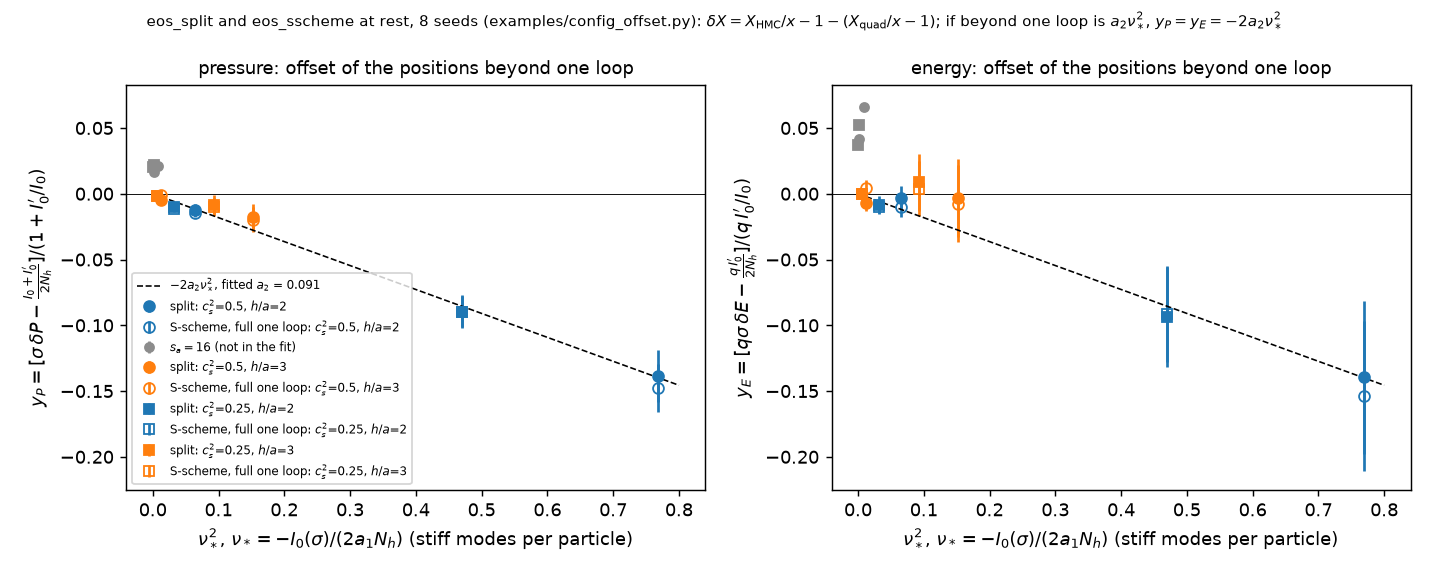
\includegraphics[width=\textwidth]{figs/config_offset_nu2.png}\end{center}
\caption{What remains of the offset of the positions after the one-loop correction, against $\nu_*^2$.  Runs \texttt{eos\_split} (filled
symbols) and \texttt{eos\_sscheme}, the full one-loop S-scheme (open symbols, $s_a=54$ and 541 only), at rest, $L=0.45$, 8 seeds of 300 updates;
\nolinkurl{examples/config_offset.py}.  Circles $c_s^2=1/2$, squares $c_s^2=1/4$; blue $h/a=2$, orange $h/a=3$; grey the lines at $s_a=16$, which are
left out of the fit.  For each line, $\delta P$ and $\delta E$ are column (1) of \Tab{tab:eoserr}, the error of hybrid Monte Carlo less the exact
single-particle error of the same scheme.  Left, the pressure:
$y_P=\big[\sigma\,\delta P-(I_0+I_0')/(2N_h)\big]/(1+I_0'/I_0)$, that is the remainder after the one-loop prediction, times $\sigma$, divided by its
factor in \Eq{a2}.  Right, the energy: $y_E=\big[q\sigma\,\delta E-qI_0'/(2N_h)\big]/(qI_0'/I_0)$.  The horizontal axis is $\nu_*^2$, with
$\nu_*=-I_0(\sigma)/(2a_1N_h)$ the number of stiff modes per particle.  If what lies beyond one loop is the term $a_2\nu_*^2$ of $\omega$, both panels
fall on the one line $y=-2a_2\nu_*^2$ (dashed), drawn with $a_2=0.091$ fitted to the 16 points at $s_a\ge54$ of split ($P$ and $E$ together,
$\chi^2/{\rm dof}=0.73$).  Error bars: the statistical error of the HMC mean, scaled in the same way.}
\label{fig:nu2}
\end{figure}

%-----------------------------------------------------------------------------
\subsection*{Level 1, amended: N4, the smoke runs (2026-11-25, interactive 62013554, worktree at 0c00611)}

\nolinkurl{examples/equilibrium.jl}, $L=0.6$ ($N=672$), $h/a=2$, $t=20$, 2 seeds (offsets 900, 901), the hybrid Monte Carlo start of 200 updates;
split, the measure form with $\beta=D/2+1$ (\texttt{sscheme}) and, at $c_s^2=1/4$, the measure form with $\beta=b=2$ (\texttt{sschemeb},
\texttt{SPH\_SSCHEME\_BETA=2}, the S-scheme coding of split).  Script \texttt{\$SCRATCH/sph/ssM/smoke\_n4\_all.sh}.  Columns: the acceptance of the
hybrid Monte Carlo start; the acceptances of the stress and residual moves of the stochastic step; KE/eq (in motion it includes the mean flow, about
15--20 for every scheme); $\Delta H/H$ at $t=20$ for the two seeds; the guard rejections per step; and for the measure form the largest fraction of
solves with $P_a<0$, the largest fraction of the proposals from the energy refused at the wall, and the smallest label at the end.
\begin{center}\scriptsize
\begin{tabular}{llll|ccc|r|r|lll}
\toprule
$c_s^2$ & $s_a$ & $v_0$ & scheme & HMC & acc.\ (stress, resid.) & KE/eq & $\Delta H/H$ & guards/step & $P_a<0$ & wall & $\min s$ \\
\midrule
1/2 & 16 & 0 & split & 0.975 & 0.927, 0.514 & 1.044 & $+7.8\,\mathrm e{-5}$, $+1.4\,\mathrm e{-5}$ & 2870 & & & \\
 & & & measure & 0.985 & 0.930, 0.506 & 1.034 & $-9.8\,\mathrm e{-5}$, $+6.5\,\mathrm e{-6}$ & 2836 & 0 & $1.1\,\mathrm e{-4}$ & 2.633 \\
 & & 0.8 & split & 0.995 & 0.962, 0.587 & 14.36 & $-1.1\,\mathrm e{-6}$, $+1.3\,\mathrm e{-7}$ & 957 & & & \\
 & & & measure & 0.995 & 0.967, 0.595 & 14.46 & $+3.3\,\mathrm e{-7}$, $-4.3\,\mathrm e{-7}$ & 782 & 0 & $7.7\,\mathrm e{-6}$ & 4.028 \\
 & 54 & 0 & split & 0.985 & 0.984, 0.854 & 0.987 & $+2.9\,\mathrm e{-5}$, $+9.7\,\mathrm e{-6}$ & 0.6 & & & \\
 & & & measure & 0.980 & 0.984, 0.852 & 0.972 & $-1.4\,\mathrm e{-5}$, $+2.3\,\mathrm e{-5}$ & 2.0 & 0 & 0 & 19.59 \\
 & & 0.8 & split & 0.990 & 0.989, 0.828 & 14.55 & $+4.9\,\mathrm e{-7}$, $-6.8\,\mathrm e{-9}$ & 0 & & & \\
 & & & measure & 0.990 & 0.989, 0.829 & 14.90 & $+1.5\,\mathrm e{-7}$, $-5.3\,\mathrm e{-7}$ & 0 & 0 & 0 & 42.74 \\
\midrule
1/4 & 16 & 0 & split & 0.970 & 0.928, 0.327 & 1.096 & $-7.6\,\mathrm e{-6}$, $+9.4\,\mathrm e{-6}$ & 2119 & & & \\
 & & & measure & 0.980 & 0.929, 0.329 & 1.060 & $+2.3\,\mathrm e{-7}$, $-1.1\,\mathrm e{-5}$ & 1927 & 0 & $8.4\,\mathrm e{-4}$ & 2.567 \\
 & & & measure, $\beta=b$ & 0.985 & 0.931, 0.355 & 1.037 & $-1.4\,\mathrm e{-5}$, $+9.1\,\mathrm e{-6}$ & 2203 & $2.2\,\mathrm e{-3}$ & $7.0\,\mathrm e{-4}$ & 2.301 \\
 & & 0.8 & split & 0.995 & 0.961, 0.445 & 18.99 & $-8.5\,\mathrm e{-8}$, $+2.1\,\mathrm e{-7}$ & 494 & & & \\
 & & & measure & 0.990 & 0.962, 0.457 & 20.76 & $+2.1\,\mathrm e{-7}$, $+8.6\,\mathrm e{-8}$ & 489 & 0 & $2.2\,\mathrm e{-4}$ & 3.222 \\
 & & & measure, $\beta=b$ & 0.985 & 0.961, 0.454 & 19.44 & $-1.4\,\mathrm e{-7}$, $-1.8\,\mathrm e{-7}$ & 526 & $1.2\,\mathrm e{-4}$ & $1.6\,\mathrm e{-4}$ & 2.423 \\
 & 54 & 0 & split & 0.970 & 0.950, 0.567 & 0.984 & $+1.1\,\mathrm e{-6}$, $+9.3\,\mathrm e{-6}$ & 20 & & & \\
 & & & measure & 0.985 & 0.949, 0.565 & 0.960 & $+7.0\,\mathrm e{-6}$, $+6.5\,\mathrm e{-6}$ & 54 & 0 & $2.1\,\mathrm e{-5}$ & 4.060 \\
 & & & measure, $\beta=b$ & 0.990 & 0.948, 0.561 & 0.972 & $+9.8\,\mathrm e{-6}$, $-1.3\,\mathrm e{-6}$ & 21 & $2.2\,\mathrm e{-6}$ & $5.0\,\mathrm e{-6}$ & 2.449 \\
 & & 0.8 & split & 1.000 & 0.969, 0.597 & 20.26 & $-1.4\,\mathrm e{-7}$, $+2.5\,\mathrm e{-8}$ & 0 & & & \\
 & & & measure & 0.995 & 0.967, 0.584 & 20.14 & $-2.0\,\mathrm e{-7}$, $-1.1\,\mathrm e{-7}$ & 0.1 & 0 & $2\,\mathrm e{-9}$ & 29.34 \\
 & & & measure, $\beta=b$ & 1.000 & 0.968, 0.591 & 19.77 & $+2.7\,\mathrm e{-7}$, $+9.6\,\mathrm e{-8}$ & 0.1 & 0 & $5\,\mathrm e{-9}$ & 27.01 \\
\bottomrule
\end{tabular}
\end{center}
\begin{itemize}
\item No solve without a state in any run (about $10^9$ solves from the label in all), and no record without a state: the fold of item E is gone.
  The hybrid Monte Carlo start accepts 0.97--1.00 for every scheme, including $s_a=16$, where the full form accepted 0.11 (item E).
\item The measure form and split agree in every column within the scatter of two seeds: the acceptances of the stochastic step, KE/eq, the drift of
  $H$ ($10^{-5}$ at $s_a=16$ at rest, $10^{-7}$ in motion, for both), and the guard rejections.
\item The wall refuses at most $8\times10^{-4}$ of the proposals from the energy ($s_a=16$, $c_s^2=1/4$, at rest), $10^{-4}$ for the conformal fluid at
  $s_a=16$, and none at $s_a=54$ for the conformal fluid.  The smallest label reached is 2.57--2.63 at $s_a=16$ at rest ($\beta=2.5$).
\item $P_a<0$: never with $\beta=D/2+1$.  With $\beta=b$ at $c_s^2=1/4$, up to $2.2\times10^{-3}$ of the solves at $s_a=16$ (the window
  $2<S_{\rm t}<2.5$ of the table of bounds in \nolinkurl{renorm3.tex}), $2\times10^{-6}$ at $s_a=54$.
\end{itemize}
\textbf{Ask} (N4): the owner reads N1 and N4 before the campaigns.

%-----------------------------------------------------------------------------
\subsection*{The next order of the single particle (2026-11-25)}

The term of order $1/S_{\rm t}$ of the label (renorm3.tex, appendix, eq.~c; constant $c_s^2$, $d=2$):
$s\to s+c(a)/S_{\rm t}$, $c=-3/8+\lambda_4/(8a^2)-5\lambda_3^2/(24a^3)$, $\lambda_3=2q(q-1)$, $\lambda_4=2q(q-1)(3q+1)$, $a=q-v^2$, with its
slopes along the modes; models \texttt{sscheme-2}, \texttt{sscheme-m-2}, \texttt{sscheme-mf-2} of \nolinkurl{examples/renorm_quadrature_sscheme.py}
(rows in \texttt{docs/figs/sscheme\_quadrature\_measure.csv}).  $E/E_{\rm t}-1$ of the single particle, $c_s^2=1/2$, at rest (in motion alike):
\begin{center}\small
\begin{tabular}{rcccc}
\toprule
$s_a$ & one loop (full form) & with the next order & the next term, $n\,c/S_{\rm t}^2$ & split \\
\midrule
541 & $9.2\times10^{-7}$ & $3.6\times10^{-8}$ & $8.5\times10^{-7}$ & $9.7\times10^{-7}$ \\
54 & $1.8\times10^{-4}$ & $5.7\times10^{-5}$ & $0.9\times10^{-4}$ & $2.4\times10^{-4}$ \\
30 & $1.9\times10^{-3}$ & $1.3\times10^{-3}$ & $2.8\times10^{-4}$ & $2.2\times10^{-3}$ \\
16 & $4.2\%$ & $3.9\%$ & $0.1\%$ & $3.9\%$ \\
\bottomrule
\end{tabular}
\end{center}
At $s_a=541$ ($v=0.8$: $2.3\times10^{-6}\to5.0\times10^{-8}$) and 54 the next order removes what it should.  At $s_a=30$ the error is already
seven times the next term and at $s_a=16$ forty times; $c_s^2=1/4$ is alike ($E$ at $s_a=16$: $8.0\%\to7.8\%$, and $p$ $7.3\%\to10\%$).  So at
$s_a\lesssim30$ the error of the single particle is not the truncation of the series in $1/S_{\rm t}$: it comes from the states near the boundary at
small $S_{\rm t}$, where the saddle point has no meaning, and it is common to every member of the family (split $3.9\%$).  A higher loop does not
reduce it; a better count of the states at small $S_{\rm t}$ (the exact series of renorm2.tex, matched to the loops above $S_{\rm t}\approx50$) might.


\paragraph{The exact count in the quadrature: why $s_a=16$ is hard} (model \texttt{exact}: one loop plus the tabulated
$\delta(S_{\rm t},\theta)=s_{\rm exact}-S_{\rm 1loop}$ of \nolinkurl{examples/exact_count.py}, \texttt{docs/figs/exact\_delta\_c*.csv}).  $E/E_{\rm t}-1$ at rest,
exact count against one loop: $c_s^2=1/2$: $3.0\%$ / $4.2\%$ ($s_a=16$), $7.5\times10^{-4}$ / $1.9\times10^{-3}$ (30), $1.7\times10^{-6}$ /
$1.8\times10^{-4}$ (54); $c_s^2=1/4$: $4.6\%$ / $8.0\%$, $3.4\times10^{-3}$ / $7.7\times10^{-3}$, $5.7\times10^{-5}$ / $5.8\times10^{-4}$.  Even the exact
count leaves 3--5\% at $s_a=16$.  The exact particle is a Poisson cloud of quanta with the mean number $\bar N=S_{\rm t}/n$, which is only 5.3
($c_s^2=1/2$) and 3.2 ($c_s^2=1/4$) at $s_a=16$.  A particle cannot be empty, so the $N=0$ state is dropped (renorm2.tex), which changes $E$ and $p$ by
$1/(e^{\bar N}-1)$; for the massless gas the states of one quantum lie on the light cone at $T=0$, where no state with a temperature represents them,
with the weight $\bar Ne^{-\bar N}$.  These give $4.3\%$ for $c_s^2=1/4$ (measured $4.6\%$) and $0.5\%+2.6\%=3.1\%$ for $c_s^2=1/2$ (measured $3.0\%$).  So
the error of the single particle at $s_a=16$ is not perturbative in $1/S_{\rm t}$: it is of order $e^{-s_a/n}$, the probability that the cell holds
no quantum or one, and no order of the loop expansion or table removes it.  It falls fast: $10^{-3}$ at $s_a=30$, $10^{-6}$--$10^{-5}$ at $s_a=54$.

\paragraph{Decision (owner, 2026-11-25).}  The main line is split with the positional counterterm ($E_{\rm dyn}=T(\Delta s_{\rm dyn}-\omega)$,
\texttt{SPH\_RENORM=split SPH\_POSITIONAL=1}).  The exact count of the single particle (\nolinkurl{examples/exact_count.py}: the Poisson cloud of
renorm2.tex in closed form, each term a Riesz kernel on the cone; $\delta=s_{\rm exact}-S_{\rm 1loop}\to c(a)/S_{\rm t}$ checked) is kept as a check
of the single particle at small $S_{\rm t}$ and is not put into the code.

%-----------------------------------------------------------------------------
\subsection*{Level 2: the positional counterterm in the Hamiltonian (2026-11-25, items H, I, J, K)}

\paragraph{The code} (commits cc86cf4, 4dda501).  \nolinkurl{src/positional.jl}: $\omega(\bar\sigma,V)=a_1\nu_*+a_2\nu_*^2$ of \Eq{omega} from the table
of $I_0$ (\nolinkurl{src/tables/i0_table_wc2.csv}, $\sigma=10^{-8}$ to $10^5$, a cubic Hermite spline in $\ln\sigma$ whose own derivative is $I_0'$),
\texttt{SPH\_POSITIONAL=1}, $a_2$ = \texttt{SPH\_POSITIONAL\_A2} (default 0).  Split: $E_{\rm dyn}=T\,(\Delta s_{\rm dyn}-\omega(u/n,V))$, the derivatives
through $T(u,|\bm m|,V)$ of the target.  The measure form: $s\to s+\omega(S_{\rm t}/n,V)$, with the slopes \Eq{slopes2}.  Off, the code is that of
level 1 bit for bit.  Tests (\nolinkurl{test/testpositional.jl}, \nolinkurl{test/testpositional_steps.jl}; both schemes, $a_2=0$, $0.091$, $0.3$): the
fields are the derivatives of $H$ to $4\times10^{-9}$, the inverse to $10^{-14}$, the label of the measure form increases with $S_{\rm t}$ (smallest
$\mathcal D$ 0.91), the Jacobian determinant of the ideal step is one to $7\times10^{-8}$, hybrid Monte Carlo at $s_a=16$ accepts 18--20 of 20 and no
trajectory leaves the domain.  At $\bar\sigma<1$, $I_0>0$ and $\omega$ is slightly negative.  Split's votes try labels $u\to0$ in their Newton
steps; the first table ($\sigma\ge0.02$) stopped four tasks there, and the table now starts at $10^{-8}$, constant below.

\paragraph{The equilibrium with $\omega$} (campaign \texttt{eos\_positional}; \Tab{tab:eoserrsw}, \Tab{tab:eoserrmw}).
\begin{table}[h]
\caption{Split with the positional counterterm in the Hamiltonian, $E_{\rm dyn}=T(\Delta s_{\rm dyn}-\omega)$ (\texttt{SPH\_RENORM=split SPH\_POSITIONAL=1}, $a_2=0$).  Campaign \texttt{eos\_positional} (interactive 62017396, commit 67471dc; the two tasks that stopped on the table of $I_0$ rerun at 4dda501), at rest, $L=0.45$, 8 seeds of 300 updates.  Columns: (0) the error of hybrid Monte Carlo, $X_{\rm HMC}/x-1$, with $\omega$ in the Hamiltonian; (1) after the exact
single-particle error of the scheme is subtracted; (p) the prediction for (1), column (2) of \Tab{tab:eoserr} (split without $\omega$, less the one-loop
correction of the positions); (3) column (1) after the term beyond one loop, $a_2\nu_*^2$ with $a_2=0.091$, is also subtracted; $\pm$ the
statistical error.  Percent.}
\label{tab:eoserrsw}
\begin{center}\small
\begin{tabular}{lrrr|rrrrr|rrrrr}
\toprule
 & & & & \multicolumn{5}{c|}{$P/p-1$ (\%)} & \multicolumn{5}{c}{$E/e-1$ (\%)} \\
$c_s^2$ & $s_a$ & $h/a$ & $\nu_*$ & (0) & (1) & (p) & (3) & $\pm$ & (0) & (1) & (p) & (3) & $\pm$ \\
\midrule
1/2 & 16 & 2 & 0.088 & $+4.36$ & $+0.45$ & $+0.86$ & $+0.51$ & 0.04 & $+5.58$ & $+1.66$ & $+1.41$ & $+1.70$ & 0.05 \\
 & 16 & 3 & 0.040 & $+4.54$ & $+0.63$ & $+0.67$ & $+0.65$ & 0.04 & $+5.03$ & $+1.11$ & $+0.88$ & $+1.12$ & 0.03 \\
 & 54 & 2 & 0.251 & $-0.17$ & $-0.19$ & $-0.11$ & $-0.08$ & 0.03 & $+0.10$ & $+0.08$ & $-0.01$ & $+0.12$ & 0.04 \\
 & 54 & 3 & 0.112 & $-0.07$ & $-0.10$ & $-0.05$ & $-0.08$ & 0.02 & $+0.01$ & $-0.01$ & $-0.03$ & $-0.00$ & 0.03 \\
 & 541 & 2 & 0.875 & $-0.13$ & $-0.13$ & $-0.11$ & $-0.01$ & 0.02 & $-0.04$ & $-0.04$ & $-0.04$ & $-0.00$ & 0.02 \\
 & 541 & 3 & 0.389 & $-0.02$ & $-0.02$ & $-0.01$ & $+0.00$ & 0.01 & $-0.00$ & $-0.00$ & $-0.00$ & $+0.01$ & 0.01 \\
\midrule
1/4 & 16 & 2 & 0.038 & $+12.49$ & $+2.12$ & $+2.12$ & $+2.15$ & 0.09 & $+12.31$ & $+3.85$ & $+3.37$ & $+3.87$ & 0.07 \\
 & 16 & 3 & 0.018 & $+12.80$ & $+2.43$ & $+1.96$ & $+2.43$ & 0.05 & $+11.43$ & $+2.97$ & $+2.40$ & $+2.98$ & 0.05 \\
 & 54 & 2 & 0.175 & $-0.10$ & $-0.34$ & $-0.17$ & $-0.25$ & 0.03 & $+0.09$ & $+0.04$ & $-0.06$ & $+0.08$ & 0.04 \\
 & 54 & 3 & 0.078 & $+0.11$ & $-0.13$ & $-0.03$ & $-0.11$ & 0.02 & $+0.06$ & $+0.00$ & $-0.00$ & $+0.01$ & 0.02 \\
 & 541 & 2 & 0.683 & $-0.14$ & $-0.14$ & $-0.12$ & $-0.02$ & 0.02 & $-0.04$ & $-0.04$ & $-0.04$ & $-0.00$ & 0.02 \\
 & 541 & 3 & 0.304 & $-0.02$ & $-0.02$ & $-0.01$ & $+0.00$ & 0.01 & $-0.00$ & $-0.00$ & $+0.00$ & $+0.01$ & 0.01 \\
\bottomrule
\end{tabular}
\end{center}
\end{table}
\begin{table}[h]
\caption{As \Tab{tab:eoserrsw} for the measure form with $\omega$ in the label ($\beta=D/2+1$ at $c_s^2=1/2$, $\beta=b$ at $c_s^2=1/4$).  Columns: (0) the error of hybrid Monte Carlo, $X_{\rm HMC}/x-1$, with $\omega$ in the Hamiltonian; (1) after the exact
single-particle error of the scheme is subtracted; (p) the prediction for (1), column (2) of \Tab{tab:eoserr} (split without $\omega$, less the one-loop
correction of the positions); (3) column (1) after the term beyond one loop, $a_2\nu_*^2$ with $a_2=0.091$, is also subtracted; $\pm$ the
statistical error.  Percent.}
\label{tab:eoserrmw}
\begin{center}\small
\begin{tabular}{lrrr|rrrrr|rrrrr}
\toprule
 & & & & \multicolumn{5}{c|}{$P/p-1$ (\%)} & \multicolumn{5}{c}{$E/e-1$ (\%)} \\
$c_s^2$ & $s_a$ & $h/a$ & $\nu_*$ & (0) & (1) & (p) & (3) & $\pm$ & (0) & (1) & (p) & (3) & $\pm$ \\
\midrule
1/2 & 16 & 2 & 0.090 & $+3.84$ & $-0.10$ & $+0.86$ & $-0.04$ & 0.04 & $+5.10$ & $+1.14$ & $+1.41$ & $+1.17$ & 0.04 \\
 & 16 & 3 & 0.040 & $+4.15$ & $+0.21$ & $+0.67$ & $+0.23$ & 0.04 & $+4.64$ & $+0.68$ & $+0.88$ & $+0.68$ & 0.04 \\
 & 54 & 2 & 0.253 & $-0.28$ & $-0.30$ & $-0.11$ & $-0.20$ & 0.05 & $+0.04$ & $+0.02$ & $-0.01$ & $+0.06$ & 0.05 \\
 & 54 & 3 & 0.113 & $-0.07$ & $-0.09$ & $-0.05$ & $-0.07$ & 0.03 & $+0.03$ & $+0.00$ & $-0.03$ & $+0.01$ & 0.03 \\
 & 541 & 2 & 0.876 & $-0.13$ & $-0.13$ & $-0.11$ & $-0.01$ & 0.02 & $-0.04$ & $-0.04$ & $-0.04$ & $-0.00$ & 0.02 \\
 & 541 & 3 & 0.389 & $-0.02$ & $-0.02$ & $-0.01$ & $+0.00$ & 0.01 & $-0.00$ & $-0.00$ & $-0.00$ & $+0.01$ & 0.01 \\
\midrule
1/4 & 16 & 2 & 0.038 & $+12.43$ & $+2.05$ & $+2.12$ & $+2.07$ & 0.07 & $+12.08$ & $+3.67$ & $+3.37$ & $+3.69$ & 0.06 \\
 & 16 & 3 & 0.018 & $+12.36$ & $+1.98$ & $+1.96$ & $+1.98$ & 0.05 & $+10.92$ & $+2.51$ & $+2.40$ & $+2.52$ & 0.05 \\
 & 54 & 2 & 0.176 & $-0.19$ & $-0.43$ & $-0.17$ & $-0.34$ & 0.06 & $+0.01$ & $-0.04$ & $-0.06$ & $-0.00$ & 0.04 \\
 & 54 & 3 & 0.079 & $+0.15$ & $-0.09$ & $-0.03$ & $-0.07$ & 0.04 & $+0.08$ & $+0.03$ & $-0.00$ & $+0.03$ & 0.03 \\
 & 541 & 2 & 0.684 & $-0.14$ & $-0.15$ & $-0.12$ & $-0.03$ & 0.02 & $-0.04$ & $-0.04$ & $-0.04$ & $-0.01$ & 0.02 \\
 & 541 & 3 & 0.304 & $-0.01$ & $-0.01$ & $-0.01$ & $+0.01$ & 0.01 & $+0.01$ & $+0.01$ & $+0.00$ & $+0.01$ & 0.01 \\
\bottomrule
\end{tabular}
\end{center}
\end{table}
\begin{itemize}
\item At $s_a\ge54$ the correction of the positions is gone: the error after the single particle, column (1), is at most $0.34\%$ in $P$ and $0.08\%$ in
  $E$, against 0.5--5\% without $\omega$, and it is what the tables without $\omega$ predict (column (p)) within one to two statistical errors.  What
  remains is the term beyond one loop: with $a_2=0.091$, column (3), at most $0.24\%$ in $P$ and $0.04\%$ in $E$ (the largest at $c_s^2=1/4$,
  $s_a=54$, $h/a=2$).
\item At $s_a=16$ the raw error (0) grows: at $c_s^2=1/2$ it is $P$ $+4.4\%$, $E$ $+5.6\%$ ($h/a=2$), against $-1.4\%$ and $+2.1\%$ without $\omega$.
  Without $\omega$ the error of the positions ($-5.3\%$ in $P$) and that of the single particle ($+3.9\%$) cancelled; with the positions corrected the
  single particle at small $S_{\rm t}$ is what is left (the next order of the series does not reduce it, \Sect{sec:results}, ``The next order'').
  At $c_s^2=1/4$ the raw error at $s_a=16$ is $+11$ to $+12.5\%$.
\item Split and the measure form agree within the errors at every line.
\end{itemize}

\paragraph{The dynamics with $\omega$} (campaign \texttt{hastings\_positional}, interactive 62017421, commit 67471dc; $c_s^2=1/2$, $L=0.6$, $h/a=2$,
$\eta/s=0.2$, at rest; \nolinkurl{examples/positional_dyn.jl}; \Fig{fig:posdyn}, \Fig{fig:posapp}).  For split+$\omega$ and the measure form+$\omega$ at
$s_a=16$ and 54: the full dynamics from the hybrid Monte Carlo start to $t=100$ (16 runs; one per split set stopped on the table and is rerun), hybrid
Monte Carlo chains of the same Hamiltonian (16), and the dynamics from the hexagonal lattice without the HMC start (8 runs).
\begin{itemize}
\item The dynamics holds the equilibrium of its own Hamiltonian: the equal-time spectra of $M_L$, $M_T$ and $E$ are those of hybrid Monte Carlo within
  2--3\% (errors 1--3\%) at $kh\le1.6$, for both schemes and both $s_a$; the largest departures are $0.94\pm0.02$ ($M_L$, $kh=0.78$, split, $s_a=16$) and
  $1.08\pm0.04$ ($M_L$, $kh=0.78$, split, $s_a=54$).  KE/eq is $1.028\pm0.006$ and $1.030\pm0.008$ at $s_a=16$, $0.996$ and $1.005$ at $s_a=54$.
\item The energy: $\Delta H/H$ at $t=100$ is $+2.0\times10^{-4}$ (split) and $+1.7\times10^{-4}$ (measure form) at $s_a=16$, the largest run $5\times10^{-4}$;
  $3$--$5\times10^{-5}$ at $s_a=54$.
\item From the lattice the positions are at equilibrium almost at once: the bond order $|\psi_6|$ falls from 1 to $0.35$ by $t=0.03$ and to its HMC value
  (0.018) by $t\approx0.06$, about one sound crossing of a lattice spacing.  The energy fluctuations, zero at the start, reach 0.9 of HMC by $t\approx0.5$.
  At $s_a=54$ every spectrum is that of HMC from $t\approx5$ on (0.97--1.0).  At $s_a=16$ they level off below it, at 0.91--0.93 (split) and 0.94--0.95
  (measure form) for $M_L$, $M_T$ and $E$ alike from $t\approx1$ to 100.  All three spectra scale as $T^4$ for the conformal fluid, so this is what a
  temperature lower by about 2\% gives: a run from the lattice keeps the energy drawn at the lattice positions, and at $s_a=16$ the positions carry
  enough energy that the microcanonical temperature differs from the bath's.  Not yet checked: the driver does not record the mean temperature.
\end{itemize}
\begin{figure}[h]
\begin{center}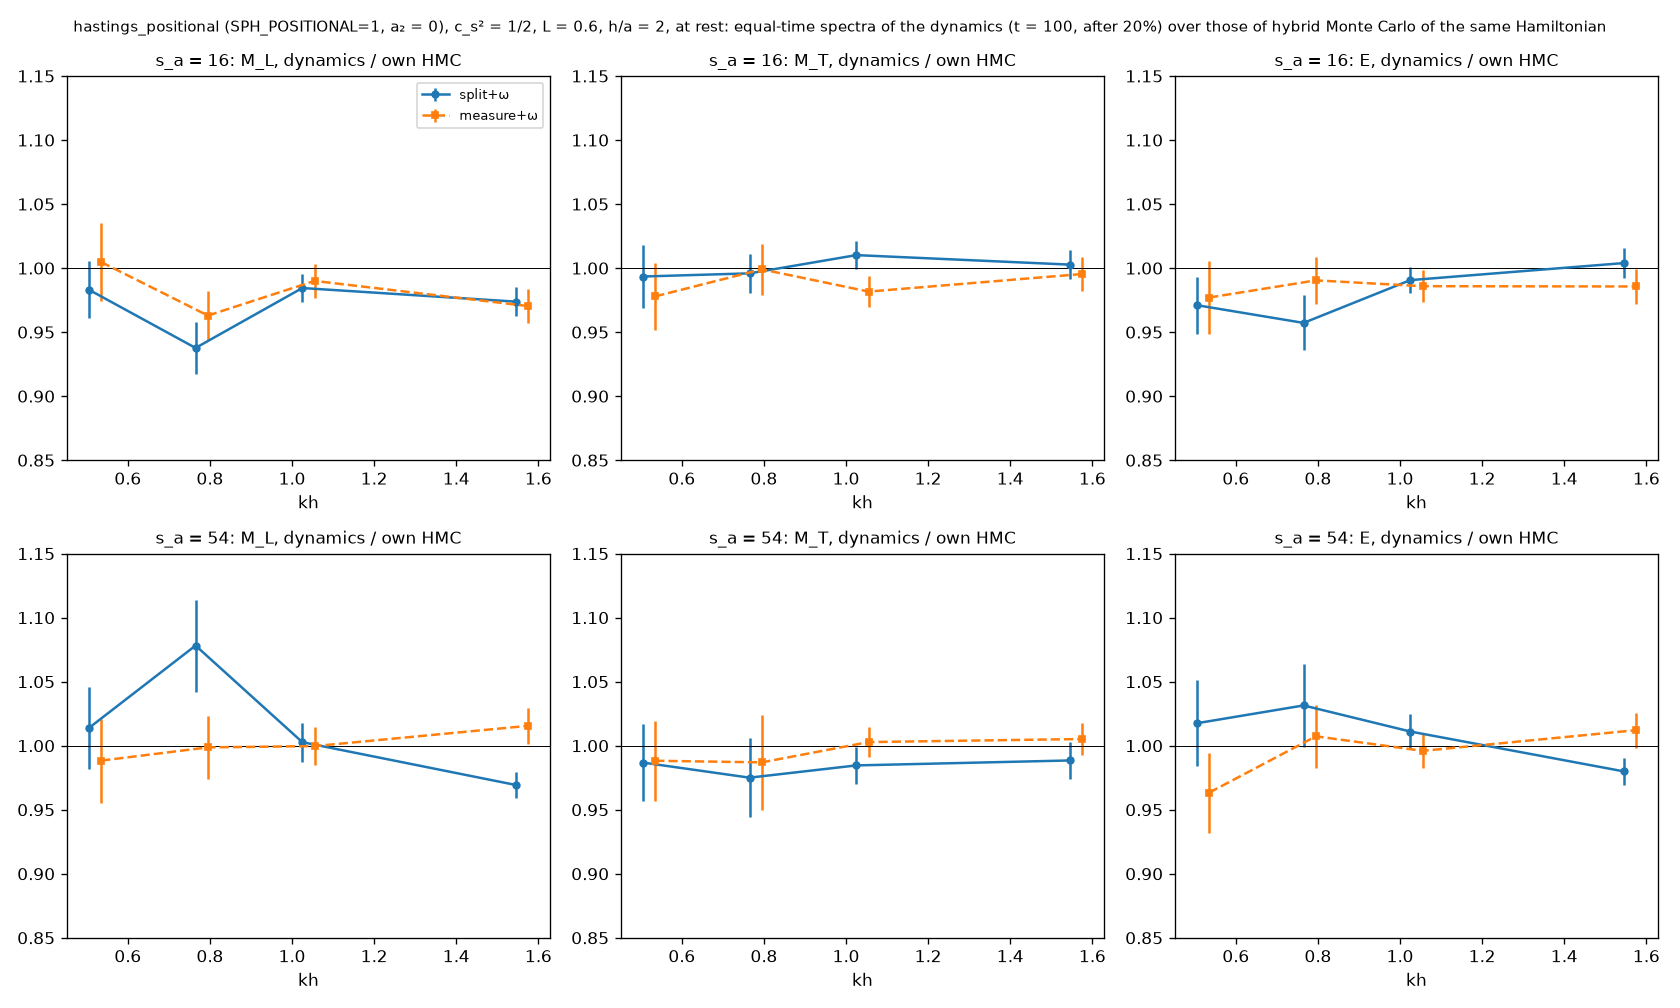
\includegraphics[width=\textwidth]{figs/positional_dyn_spectra.png}\end{center}
\caption{Campaign \texttt{hastings\_positional}: the equal-time spectra $|M_{L,k}|^2/N$, $|M_{T,k}|^2/N$ and $|E_k-\langle E_k\rangle|^2/N$ of the dynamics
from the hybrid Monte Carlo start (records after 20\% of $t=100$), divided by those of hybrid Monte Carlo chains of the same Hamiltonian (after 20
updates), in bands of $kh$ of width 0.26; split with $\omega$ in the energy (circles) and the measure form with $\omega$ in the label (squares);
$c_s^2=1/2$, $s_a=16$ (top) and 54 (bottom).  Errors from the spread between runs.}
\label{fig:posdyn}
\end{figure}
\begin{figure}[h]
\begin{center}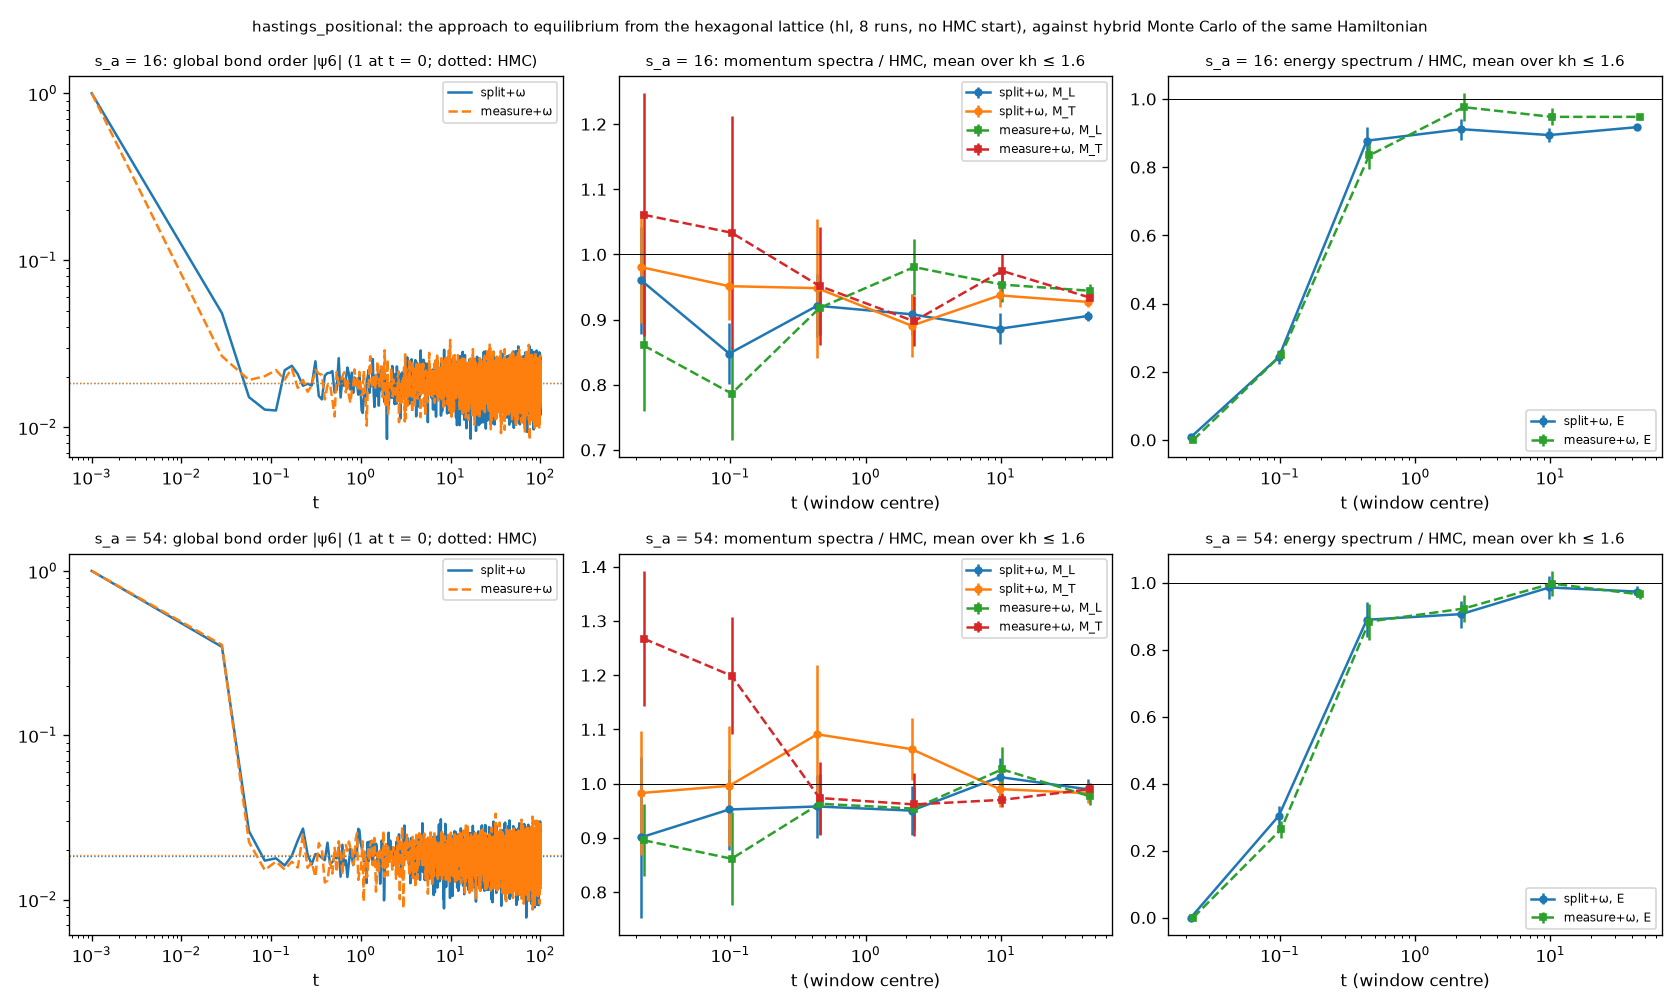
\includegraphics[width=\textwidth]{figs/positional_dyn_approach.png}\end{center}
\caption{Campaign \texttt{hastings\_positional}: the approach to equilibrium from the hexagonal lattice (8 runs each, no hybrid Monte Carlo start).
Left: the global bond order $|\psi_6|$ (1 on the lattice at $t=0$), dotted its value in hybrid Monte Carlo.  Middle and right: the spectra of $M_L$, $M_T$
and $E$ averaged over $kh\le1.6$ in windows of $t$ ($[0,0.05]$, $[0.05,0.2]$, $[0.2,1]$, $[1,5]$, $[5,20]$, $[20,100]$, plotted at the geometric centre),
divided by hybrid Monte Carlo of the same Hamiltonian; errors from the spread between runs.}
\label{fig:posapp}
\end{figure}

%-----------------------------------------------------------------------------
\section{The exact form: all of the renormalization in the label (2026-11-26, branch \texttt{sscheme-measure})}
\label{sec:exact}

\paragraph{The idea (owner, 2026-11-26).}  The exact count of the states of one particle (\nolinkurl{examples/exact_count.py}, ``The exact count in
the quadrature'' above) cuts the dynamics off at small $S_{\rm t}$ in a natural way, so it is put into the label, as the S-scheme first meant to do:
\st
s=s_{\rm exact}(e,\bm m,V)=\ln G(e,|\bm m|,V)-\ln V-1=S_{\rm 1loop}+\delta(\ln S_{\rm t},\theta)\,,\qquad S_{\rm 1loop}=S_{\rm t}-\Delta_\chi-\Delta_\ell\,,
\label{sexact}
\stp
with the flat Liouville measure $e^s\,ds\,d^2m\,d^2x$: no wall, no $\beta\ln S_{\rm t}$ in the measure, no reference state.  $\theta$ is the rapidity
of the target and $\delta$ depends on $(S_{\rm t},\theta)$ alone (the constant $A$ of $p=AT_{\rm rel}^n$ cancels).  Two properties make it the natural
cutoff.  The exact number of states increases with the energy at every $(\bm m,V)$, so $s(e)$ has no fold (the one loop folds at $S_{\rm t}\approx b$,
\Sect{sec:results}, E).  And as $S_{\rm t}\to0$ the count is that of one quantum, so for $c_s^2=1/2$ the label has a floor,
\st
s\to s_{\rm min}=\ln\!\big(A\,K(\tfrac n2)\big)-1=\ln\frac{A}{2\pi}-1\,,
\stp
with $K$ the constant of the Riesz kernel.  Labels below it have no state, and near it $\partial s/\partial e\to0$ and $T_a=\partial H/\partial s\to\infty$:
a particle cannot be emptied.  The single-particle error that is left is the $N=0$ state and the light cone (3\% at $s_a=16$, $10^{-6}$ at $s_a=54$,
above), which no label removes.  The positional counterterm enters as before, $s\to s+\omega(S_{\rm t}/n,V)$.  The comparison in the dynamics is
split$+\omega$ against the exact form$+\omega$ (\nolinkurl{split_dynamics.tex}, campaign \texttt{hastings\_compare}).

\paragraph{The steps and their checks.}
\begin{enumerate}
\item[X1.] \emph{The table.}  \texttt{python3 examples/exact\_count.py dyntable}: $\ell=\ln g$, $g=s_{\rm exact}-s_{\rm min}$ at $A=V=1$, on
  $x=\ln S_{\rm t}\in[\ln10^{-3},\ln10^6]$ (step 0.05) and $\theta\in[0,6]$ (step 0.1), $c_s^2=1/2$: the exact count up to $S_{\rm t}=600$, above it
  $S_{\rm 1loop}+c(a)/S_{\rm t}+d(\theta)/S_{\rm t}^2$ with $d$ matched at 600.  The nodal derivatives $\ell_x,\ell_\theta,\ell_{x\theta}$ are those of a
  bicubic spline through the values, the grid mirrored in $\theta$ ($g$ is even), in \texttt{src/tables/exact\_lng\_c05.csv}.  Why $\ln g$: as
  $S_{\rm t}\to0$, $g\propto S_{\rm t}^3$ ($9\times10^{-12}$ at $S_{\rm t}=10^{-3}$), so a table of $\delta=s_{\rm exact}-S_{\rm 1loop}\approx-17$ there
  (the first try) cannot give $\mathcal D=\partial s/\partial S_{\rm t}$ (a difference of numbers near one) and made spurious folds; $\ell$ is linear in
  $x$ there with slope 3.  Check (\texttt{checkpoints}, 85 points off the grid, $10^{-3}\le S_{\rm t}\le600$): the interpolant gives the exact
  label to $3\times10^{-7}$ (the largest at $S_{\rm t}\approx2$--8, where $\ell$ curves most) and its slopes to $5\times10^{-6}$.
\item[X2.] \emph{The label in the code} (\texttt{SPH\_SSCHEME\_FORM=exact}, \nolinkurl{src/sscheme_exact.jl}).  For the conformal fluid the label is a
  function of $(S_{\rm t},\theta)$ alone, plus $\ln A$:
  \st
  s=s_{\rm min}+\ln A+g(\ln S_{\rm t},\theta)\ (+\,\omega)\,,
  \stp
  with $g$ from a bicubic Hermite interpolant of $\ell$ (C$^1$: the forces are derivatives of one $H$); outside the table $\ell$ is linear in $x$ and
  $\theta>6$ is clamped.  The state follows from the slopes $G_x=\partial s/\partial x$, $G_\theta=\partial s/\partial\theta|_x$ directly, with no one-loop
  parts to cancel:
  \st
  \begin{gathered}
  y=\frac{aG_x-vG_\theta}{aS_{\rm t}}\,,\quad z=\frac{vG_x+G_\theta}{S_{\rm t}}\,,\quad\mathcal D=(1+v^2)y-vz\,,\\
  T_a=\frac T{\mathcal D}\,,\quad v_a=\frac{2vy-z}{\mathcal D}\,,\quad\frac{P_aV}{T_a}=\frac{G_x}n+\omega_V\,,
  \end{gathered}
  \stp
  the relations of the S-scheme with $\Delta=S_{\rm t}-s$ (at rest $\mathcal D=G_x/S_{\rm t}$, $P_aV/T_a=G_x/n$).  There is no wall: every $S_{\rm t}>0$
  has a state.  Checks (\texttt{test/testsscheme\_exact.jl}): the interpolant; the edges; $\partial H/\partial s=T_a$, $\partial H/\partial\bm m=\bm v_a$,
  $\partial H/\partial V=-P_a$ by differences from $S_{\rm t}=0.5$ to 2000 (to $10^{-10}$--$10^{-8}$); the inverse maps; no fold on a dense grid
  ($S_{\rm t}=0.5$--$10^5$, $\theta\le5.2$: smallest $\mathcal D=0.0069$ at $S_{\rm t}=0.5$); the floor; $\bm v_a=0$ at $\bm m=0$.
\item[X3.] \emph{The steps.}  The Jacobian of the ideal step (\texttt{testsscheme\_jacobian.jl}), hybrid Monte Carlo at $s_a=16$
  (\texttt{testsscheme\_hmc.jl}), $\omega$ with the exact form (\texttt{testpositional.jl}, \texttt{testpositional\_steps.jl}), and the full suite
  (\texttt{test/run.sh all}) for the defaults.
\item[X4.] \emph{Smoke runs} at NERSC: the dynamics and hybrid Monte Carlo at $s_a=16$ and 54, at rest and $v_0=0.8$, with the counters (no state,
  the wall, bisections) and $\Delta H/H$.
\item[X5.] \emph{The equation of state}: hybrid Monte Carlo with $\omega$ against the quadrature of the model \texttt{exact}, as in the tables of level 2.
  The single particle is the model \texttt{exact} as computed before (one loop plus the table of $\delta$ for $S_{\rm t}\ge0.5$): its states below
  $S_{\rm t}=0.5$ carry a negligible weight at $s_a\ge16$ (the dynamics at $s_a=16$ never goes below $S_{\rm t}\approx0.8$).  The model computed from the
  table of the dynamics down to $S_{\rm t}\to0$ breaks the quadrature (its Gaussian grid in $(\ln T,\bm\eta)$ around one peak cannot hold the states of
  one quantum on the light cone, $T\to0$, $v\to1$): not needed here, to be redone with a grid for that corner if wanted.
\item[X6.] \emph{The dynamics}: the lines of \texttt{hastings\_compare} for the exact form$+\omega$, against split$+\omega$.
\end{enumerate}

\paragraph{Results.}
\begin{itemize}
\item X1, X2 (debug 62047724 for the table and its checks): all pass, as above.
\item X3 (debug 62048441): the Jacobian of the ideal step at fixed labels, $\ln\det J=6\times10^{-8}$ ($N=168$, $s_a=16$); hybrid Monte Carlo at
  $s_a=54$ and 16: $|\Delta H/H|$ falls as $\delta t^2$ (ratio 16.1), 19 of 20 updates accepted at $s_a=16$, $9\times10^4$ solves from the label with 1.7
  Newton steps each and no fallback and no solve without a state; with $\omega$: the derivatives of $H$ to $10^{-10}$, the inverse maps, the Jacobian
  ($8\times10^{-8}$) and hybrid Monte Carlo (19 of 20).  The smallest label in the HMC chains at $s_a=16$ is $-3.5$, near the floor
  ($s_{\rm min}+\ln A$).
\item X4, smoke runs (debug 62049195, commit 14ce681, \nolinkurl{nersc/smoke_x4_sscheme_exact.sh}; $c_s^2=1/2$, $L=0.6$, $h/a=2$, $t=20$, 2 seeds; the exact
  form without and with $\omega$, split$+\omega$ as the reference; hybrid Monte Carlo of the exact form$+\omega$, 60 updates).  No solve without a state
  and one bisection in about $10^9$ solves from the label (2.1 Newton steps each); no state refused.  $|\Delta H/H|$ at $t=20$: $\le6\times10^{-5}$ at
  $s_a=16$ at rest, $\le3\times10^{-5}$ at $s_a=54$ at rest, $\le2\times10^{-6}$ in motion, as split$+\omega$ ($2\times10^{-6}$--$2\times10^{-4}$ and
  $\le7\times10^{-7}$).  Hybrid Monte Carlo accepts 0.97--1.0.  At $s_a=16$ at rest the particles go down to $S_{\rm t}\approx0.8$ (labels $-3.6$, near the
  floor) without trouble: the cutoff works as intended.  Differences from split$+\omega$, at $s_a=16$ at rest only: the acceptances of the stochastic
  step are lower, $(0.82$--$0.85,\ 0.40$--$0.42)$ for the stress and the residual move against $(0.93,\ 0.52$--$0.54)$, and with $\omega$ a fraction
  $2.4\times10^{-3}$ of the solves have $P_a<0$ (none without $\omega$; $8\times10^{-5}$ in motion).  The smallest particles have $\mathcal D\to0$, a
  large $T_a$, and a small or negative pressure where $\omega_V<0$ ($\nu_*<0$ at small $\bar\sigma$); presumably the votes that move entropy into or out of them are rejected more often (not yet checked).  At $s_a=54$
  the two are indistinguishable (acceptances $(0.98,\ 0.85)$ both).
\item X5, the equation of state (interactive 62049406, 12 minutes on 2 nodes, campaign \texttt{eos\_positional}, lines \texttt{eosP\_ssx},
  \nolinkurl{nersc/campaign_eos_positional_ssx.txt}; \nolinkurl{examples/config_offset.py}).  Hybrid Monte Carlo of the exact form$+\omega$ at rest, $c_s^2=1/2$,
  $L=0.45$, 8 seeds of 300 updates; the error $X_{\rm HMC}/x-1$ in percent, (0) raw, (1) less the single particle of the model \texttt{exact}:
  \begin{center}
  \begin{tabular}{rrcccccc}
  \toprule
  $s_a$ & $h/a$ & $P$ (0) & $P$ (1) & $E$ (0) & $E$ (1) & split$+\omega$: $P$ (0) & $E$ (0) \\
  \midrule
  16 & 2 & $+2.96$ & $-0.00$ & $+3.73$ & $+0.74$ & $+4.36$ & $+5.58$ \\
  16 & 3 & $+3.02$ & $+0.05$ & $+3.30$ & $+0.30$ & $+4.54$ & $+5.03$ \\
  54 & 2 & $-0.22$ & $-0.22$ & $-0.01$ & $-0.01$ & $-0.17$ & $+0.10$ \\
  54 & 3 & $-0.07$ & $-0.07$ & $-0.02$ & $-0.02$ & $-0.07$ & $+0.01$ \\
  541 & 2 & $-0.13$ & $-0.13$ & $-0.04$ & $-0.04$ & $-0.13$ & $-0.04$ \\
  541 & 3 & $-0.02$ & $-0.02$ & $-0.00$ & $-0.00$ & $-0.02$ & $-0.00$ \\
  \bottomrule
  \end{tabular}
  \end{center}
  Errors $\le0.09\%$.  At $s_a=16$ the exact form's raw error is 1.4--1.9 points smaller than split$+\omega$'s; what is left after its single particle
  (the empty cell and the light cone, 3\%) is $\le0.74\%$.  At $s_a\ge54$ the two agree.
\item X6, the dynamics (interactive 62049405, 23 minutes on 4 nodes; \nolinkurl{split_dynamics.tex}, ``The exact form of the S-scheme against split'').  The
  exact form$+\omega$ samples its own equilibrium as split$+\omega$ does; the sound at $s_a=16$ at rest is in phase ($1.018\pm0.004$, where the measure
  form$+\omega$ gave 1.36); $\Delta H/H$ rises slowly at $s_a=16$ at rest ($+1.9\times10^{-4}$ by $t=100$, four times split$+\omega$), and the shear mode at rest at
  $s_a=16$ is more damped (6.1 against 4.4--5.1 times hydrodynamics); at $s_a=54$ the two cannot be told apart.  In the HMC chains at $s_a=16$ some trajectories
  leave the domain and are rejected (9 of 16 chains at rest, 4 of 16 in motion have one; acceptance 0.98), none at $s_a=54$.
\end{itemize}

%=============================================================================
\section{The choice of \texorpdfstring{$\beta$}{beta} off conformal: the pressure of the label gas (2026-11-26)}
\label{sec:beta}

\paragraph{The question (owner, 2026-11-26).}  For the conformal fluid the measure forms with $\beta=b$ and $\beta=D/2+1$ are the same.  Off
conformal they differ, and they seem to make different choices: $\beta=b$ takes its reference from the volume ($\bar V$), $\beta=D/2+1$ from the
temperature ($T_0$).  But there are many ways to name the reference; the $\beta=b$ case could as well be written with a reference temperature, like
$\beta=D/2+1$ (owner).  And the code sets \texttt{T\_scale}$\,=1$ everywhere.  Can the choice be stated once, through the pressure of the gas of
labels?  This section answers on paper, with one numerical check of the maps.  No campaign has been run.

\paragraph{The one loop and its scale.}  With $D=d+1$, a constant speed of sound, $q=1/c_s^2$, $n=q+1$, and
\st
b=\frac D2+d\,c_s^2,\qquad \mathcal N=1-d\,c_s^2=\frac D2+1-b,
\stp
the one-loop counterterm of the particle is, with $S_{\rm t}=\gamma s_{\rm rel}V$,
\st
\Delta=\Big(\frac D2+1\Big)\ln S_{\rm t}-\mathcal N\ln\frac{s_{\rm rel}}{s_*}+\tfrac12\ln\big(1-c_s^2v^2\big)
=b\ln S_{\rm t}+\mathcal N\ln\frac{\gamma V}{V_*}+\tfrac12\ln\big(1-c_s^2v^2\big) .
\label{deltascale}
\stp
$S_{\rm t}$ is a number, but $s_{\rm rel}$ and $V$ are not, so off conformal the count carries a scale, $s_*=1/V_*$, set by $A$ (that is, by
\texttt{T\_scale}, through $\hbar$).  For the conformal fluid $\mathcal N=0$ and the scale drops out.

\paragraph{One family.}  The measure form puts $\beta\ln s$ into the measure of the labels, $\rho(s)=e^s s^{-\beta}(1-\beta/s)$, and keeps
$\Delta^H=\Delta-\beta\ln S_{\rm t}-{\rm const}$ in the label, with the constant fixed by the reference state, $\Delta^H(\bar S_{\rm t})=0$.  Write
\st
\beta=b+\lambda\,\mathcal N:\qquad
\Delta^H=(1-\lambda)\,\mathcal N\ln\frac{\gamma V}{\bar V}-\lambda\,\mathcal N\ln\frac{s_{\rm rel}}{\bar s_{\rm rel}}+\tfrac12\ln\big(1-c_s^2v^2\big) .
\label{betafamily}
\stp
$\lambda=0$ is $\beta=b$ (the volume only, reference $\bar V$), and $\lambda=1$ is $\beta=D/2+1$ (the temperature only, since
$\mathcal N\ln s_{\rm rel}=(q-d)\ln T_{\rm rel}+{\rm const}$; reference $T_0$, \Eq{amend}).  The two choices are two points on one line.

\paragraph{The reference is one state, whatever the $\beta$.}  The reference only fixes the constant of $\Delta^H$.  In the form the code uses,
\st
\Delta^H=\Big(\frac D2+1-\beta\Big)\ln\frac{S_{\rm t}}{\bar S_{\rm t}}-\mathcal N\ln\frac{s_{\rm rel}}{\bar s_{\rm rel}}+\tfrac12\ln\big(1-c_s^2v^2\big),
\qquad \bar S_{\rm t}=\bar s_{\rm rel}\bar V,
\stp
it is one state of the particle, $(\bar S_{\rm t},\bar s_{\rm rel})$, or equivalently $(\bar S_{\rm t},T_0)$ with $\bar s_{\rm rel}=s_{\rm rel}(T_0)$,
for every $\beta$.  For $\beta=b$ the combination that appears is $\bar V=\bar S_{\rm t}/s_{\rm rel}(T_0)$, so the volume is not a separate choice: it
can be named by a reference temperature and the nominal entropy per particle, as for $\beta=D/2+1$.  For $\beta=D/2+1$ the term in $\bar S_{\rm t}$
drops and $T_0$ alone is left; for $\beta_*$ below it is $\bar p\bar V$.  One convention covers all of them: the reference is the nominal state of the
run, $T_0=T_{\rm rel,0}$ from \texttt{SR\_SREL0} and $\bar S_{\rm t}=s_a$.  (The code takes $\bar s_{\rm rel}$ as the mean of the targets of the initial
condition and $\bar V=L^2/N$, which is that state up to the fluctuations of the start.)  What distinguishes the members is not the reference but the
function the remainder depends on: $\gamma V$, $T_{\rm rel}$, or, below, the energy.

\paragraph{Who carries the pressure.}  At fixed energy, $\partial\ln S_{\rm t}/\partial\ln V=p/(e+p)=1/n$.  Moving $\beta\ln S_{\rm t}$ out of $\Delta$
therefore adds $\beta/n$ to $P_aV/T_a$ from the Hamiltonian, and the label gas, through $s^{-\beta}$, carries
\st
\frac{P_{\rm label}V}{T_a}=-\frac\beta n\quad\text{per particle.}
\stp
The total does not depend on $\beta$; $\beta$ decides how it is shared.  What the Hamiltonian carries (plain form, $F=1$) is
\st
\frac{P_aV}{T_a}=\frac{S_{\rm t}}n-\mathcal N+\frac{\lambda\mathcal N}n ,
\label{betapressure}
\stp
the tree level $S_{\rm t}/n$ plus the part of the remainder $\Delta^H$.  For $\lambda=1$ this is \Eq{amendstate}, $(S_{\rm t}-(q-d))/n$.

\paragraph{The rule from the pressure.}  Ask that the remainder in the Hamiltonian carry no pressure, so that the label gas carries all of the
one-loop pressure.  This is $\lambda=n$:
\begin{keyeq}
\st
\beta_*=b+n\mathcal N=\frac D2+1+q-d,\qquad
\Delta^H=-q\mathcal N\ln\frac{\gamma pV}{\bar p\bar V}+\tfrac12\ln\big(1-c_s^2v^2\big),\qquad \frac{P_a}{T_a}=\frac{P_{\rm tree}}{T_{\rm tree}} .
\label{betastar}
\stp
\end{keyeq}
At rest $\gamma pV=E/q$: the remainder is a function of the energy of the particle alone, and the reference is one energy, $\bar E$, in place of
$\bar V$ or $T_0$.  The three values in $d=2$:
\begin{center}
\begin{tabular}{lccc}
\toprule
$c_s^2$ & $\beta=b$ & $\beta=D/2+1$ & $\beta_*$ \\
\midrule
$1/2$ & $5/2$ & $5/2$ & $5/2$ \\
$1/3$ & $13/6$ & $5/2$ & $7/2$ \\
$1/4$ & $2$ & $5/2$ & $9/2$ \\
\bottomrule
\end{tabular}
\end{center}
The cost of $\beta_*$ is a larger exponent and a higher bound of the measure, $s>\beta_*$.  In exchange the pressure cannot go negative: by \Eq{pastar} below, $P_a=p/\mathcal D>0$ wherever $\mathcal D>0$
(compare \Sect{sec:amend}, ``The bounds to expect'').  Whether $\mathcal D>0$ (no fold) holds everywhere above the bound has not been checked.

\paragraph{What $T$, $p$, $T_a$ and $P_a$ are.}  The target of a particle is the uniform fluid cell, at tree level, with the particle's energy
$e=H$, momentum $\bm m$ and volume $V$:
\st
e=V\big(w\gamma^2-p\big),\qquad \bm m=w\gamma^2\bm v\,V,\qquad w=e_{\rm rel}+p=T_{\rm rel}s_{\rm rel},\qquad S_{\rm t}=\gamma s_{\rm rel}(T_{\rm rel})V ,
\stp
which gives the rest-frame temperature $T_{\rm rel}$ and the velocity $\bm v$ of the target (\texttt{sscheme\_target\_entropy}).  $T=T_{\rm rel}/\gamma$
is its lab-frame temperature and $p=p(T_{\rm rel})=AT_{\rm rel}^{\,n}$ its pressure; since $p=s_{\rm rel}T_{\rm rel}/n$, $pV/T=S_{\rm t}/n$.  $T_a$
and $P_a$ belong to the dynamics: they are the derivatives of the Hamiltonian $H(s,\bm m,V)$ at fixed label,
\st
T_a=\frac{\partial H}{\partial s}=\frac T{\mathcal D},\qquad P_a=-\frac{\partial H}{\partial V},\qquad \mathcal D=\frac{\partial s}{\partial S_{\rm t}} .
\stp
With \Eq{betapressure}, for any $\beta=b+\lambda\mathcal N$ (plain form),
\st
P_a=\frac1{\mathcal D}\Big[p-\Big(1-\frac\lambda n\Big)\mathcal N\,\frac TV\Big],
\qquad\text{and at }\beta_*:\qquad P_a=\frac p{\mathcal D},\quad T_a=\frac T{\mathcal D} .
\label{pastar}
\stp
At $\beta_*$ the pressure and the temperature of the dynamics are those of the target, both divided by the same $\mathcal D$, at every velocity.
\begin{itemize}
\item For the conformal fluid $\mathcal N=0$, so $P_a=p/\mathcal D$ holds for every $\beta$: all S-scheme runs so far without $\omega$ have it.
\item The positional counterterm adds $\omega_V T_a/V$ to $P_a$ (level 2), so with $\omega$ it holds at no $\beta$.
\item The velocity is not that of the target: $v_a=(v(\kappa-2\epsilon_p)+\epsilon_\parallel)/\mathcal D$ (\Eq{amendstate}) carries the slope of
  $\Delta^H$ in the rapidity, from $\tfrac12\ln(1-c_s^2v^2)$ and from $\gamma$ in $\gamma pV$.
\end{itemize}

\paragraph{What $\beta_*$ does not say.}  It does not make the single particle the infinite-volume one.  That is the condition that fixes the
counterterm $\Delta$, at one loop, and it holds for every $\beta$, since $\beta$ only moves pressure between $H$ and the label gas.  $\beta_*$ says
something narrower: the equation of state holds particle by particle in the mechanics, $P_a/T_a=p/T$ at the target, and the one-loop correction
of the pressure lives entirely in the statistics of the labels, the factor $s^{-\beta_*}$.  The conformal runs show that this is not the whole
story: they have $P_a=p/\mathcal D$, yet at $s_a=16$, $h/a=2$ the measure form without $\omega$ is off by $P$ $-1.4\%$, $E$ $+2.1\%$ against hybrid
Monte Carlo (Results, ``Level 2: the positional counterterm in the Hamiltonian''), from the positions, the light cone and beyond one loop.  Off conformal there are already data at
$c_s^2=1/4$ (Results, ``The correction of the positions: one loop and $\nu_*$''): $\beta=b$ gives split's numbers at every $s_a$, and $\beta=D/2+1$ is worse at $s_a=16$ ($E$ raw $+8.2\%$
against $+7.4\%$).  On \Eq{betafamily}, $\beta_*$ lies beyond $\beta=D/2+1$ from $\beta=b$ ($\lambda=n$ against 1 and 0), so that trend is a warning
for $\beta_*$, to be tested.

\paragraph{Check.}  \Eq{betapressure} against the maps of \nolinkurl{src/sscheme.jl} (measure form, \texttt{SPH\_SSCHEME\_BETA} set to each
value, an arbitrary reference $\bar s_{\rm rel}=3$, $\bar V=4$): $P_aV/T_a-S_{\rm t}/n$ at $S_{\rm t}=16$, 54 and 541, at rest:
\begin{center}
\begin{tabular}{lccc}
\toprule
$c_s^2$ & $\beta=b$ & $\beta=D/2+1$ & $\beta_*$ \\
\midrule
$1/4$, predicted $-\mathcal N+\lambda\mathcal N/n$ & $-0.5$ & $-0.4$ & $0$ \\
$1/4$, the maps & $-0.500000$ & $-0.400000$ & $0.000000$ \\
$1/3$, predicted & $-0.3333$ & $-0.25$ & $0$ \\
$1/3$, the maps & $-0.333333$ & $-0.250000$ & $0.000000$ \\
\bottomrule
\end{tabular}
\end{center}
The same holds in motion: at $c_s^2=1/3$ with $|\bm m|=0.4\,S_{\rm t}$ ($v=0.38$, 0.21, 0.15 at the three $S_{\rm t}$) the maps give $-0.333333$,
$-0.250000$ and $0.000000$, as predicted: the remainder at $\beta_*$ carries no pressure at any velocity, since $\tfrac12\ln(1-c_s^2v^2)$ has no
slope along $\ln V$ or $\ln T_{\rm rel}$.  (A scratch script on the login node, seconds; not a test of the suite.)

\paragraph{The scale and \texttt{T\_scale}$\,=1$.}
\begin{itemize}
\item At tree level \texttt{T\_scale} is a unit of energy.  At fixed $s_{\rm rel}$ and $V$, changing it scales $E$, $\bm m$ and $T$ together and
  leaves the trajectories and the entropies unchanged.
\item In the forms with the flat measure (full, exact) the scale enters only as a constant added to the label, through $\ln A$, and $e^s\,ds$ does
  not see it.  For the conformal exact form this is the $\ln A$ of $s=s_{\rm min}+\ln A+g$.
\item In the measure form $s^{-\beta}$ is not invariant under a shift of $s$, so the constant matters, at relative order
  $\beta\mathcal N\ln(\text{ratio of scales})/S_{\rm t}^2$ in $T_a$ and $P_a$ (not computed).  The code fixes it with the reference state of the run
  instead of $A$, which makes $s\approx S_{\rm t}$ where the particles are.
\item The scale becomes physical only beyond one loop for a non-conformal exact count, where it sets the number of quanta per unit of entropy.
\end{itemize}
So \texttt{T\_scale}$\,=1$ is harmless for what has been run.  The weakness of the present choice is elsewhere: the reference is taken from the
initial condition, which is right in equilibrium but goes stale in an expanding flow, with an error of order $\mathcal N\ln(V/\bar V)/S_{\rm t}$.

\paragraph{For the owner.}  (i) Whether to keep $\beta=b$, $\beta=D/2+1$, $\beta_*$, or the whole family as one setting, when the code is pruned.
(ii) The non-conformal run (split$+\omega$ against the measure form at $\beta=b$, $D/2+1$ and $\beta_*$, $s_a=16$ and 54, at rest and $v_0=0.8$),
estimated at 5--7 node-hours, waits for that decision; before it, the tests of the S-scheme and of $\omega$ need a pass at $c_s^2=1/3$ (they cover
$1/2$ and $1/4$).

\end{document}
